\chapter{Two-dimensional guide-vane sections}
\label{app:gv_2d_sections}
\fancyhead{}

This appendix collects the two-dimensional section stacks of all 18 active guide-vane configurations of the screening matrix (Table~\ref{tab:design_matrix}). Each plot shows the unwrapped vane sections in the axial-tangential plane across the design span $r \in [0.12,\,0.25]$~m, produced by the parametric MATLAB tool \texttt{vanedesign\_loft\_export}~\cite{Leonsen2025} before the cylindrical wrapping step described in Section~\ref{sec:theory_geometric_construction}. The section outlines are shaded by radius, from the inner cut-out (light) to the shroud (dark). The three-dimensional renderings of the same configurations are collected in Appendix~\ref{app:gv_3d_geometries}.

The two chord-control strategies are visible directly. In the constant-chord (CC) family every section keeps the same chord, so the outlines overlap closely along the span. In the constant-solidity (CS) family the chord scales with radius, so the sections taper inwards and fan out from the shroud towards the inner cut-out (Section~\ref{sec:theory_const_chord_const_sol}).

The figures are grouped by design family. The constant-chord (CC) family is presented first, followed by the constant-solidity (CS) family. Within each family, the cases are ordered by ascending shroud chord and then by ascending vane count.

\section*{Constant-chord (CC) family}

\begin{figure}[H]
  \centering
  \begin{subfigure}[b]{0.48\textwidth}
    \centering
    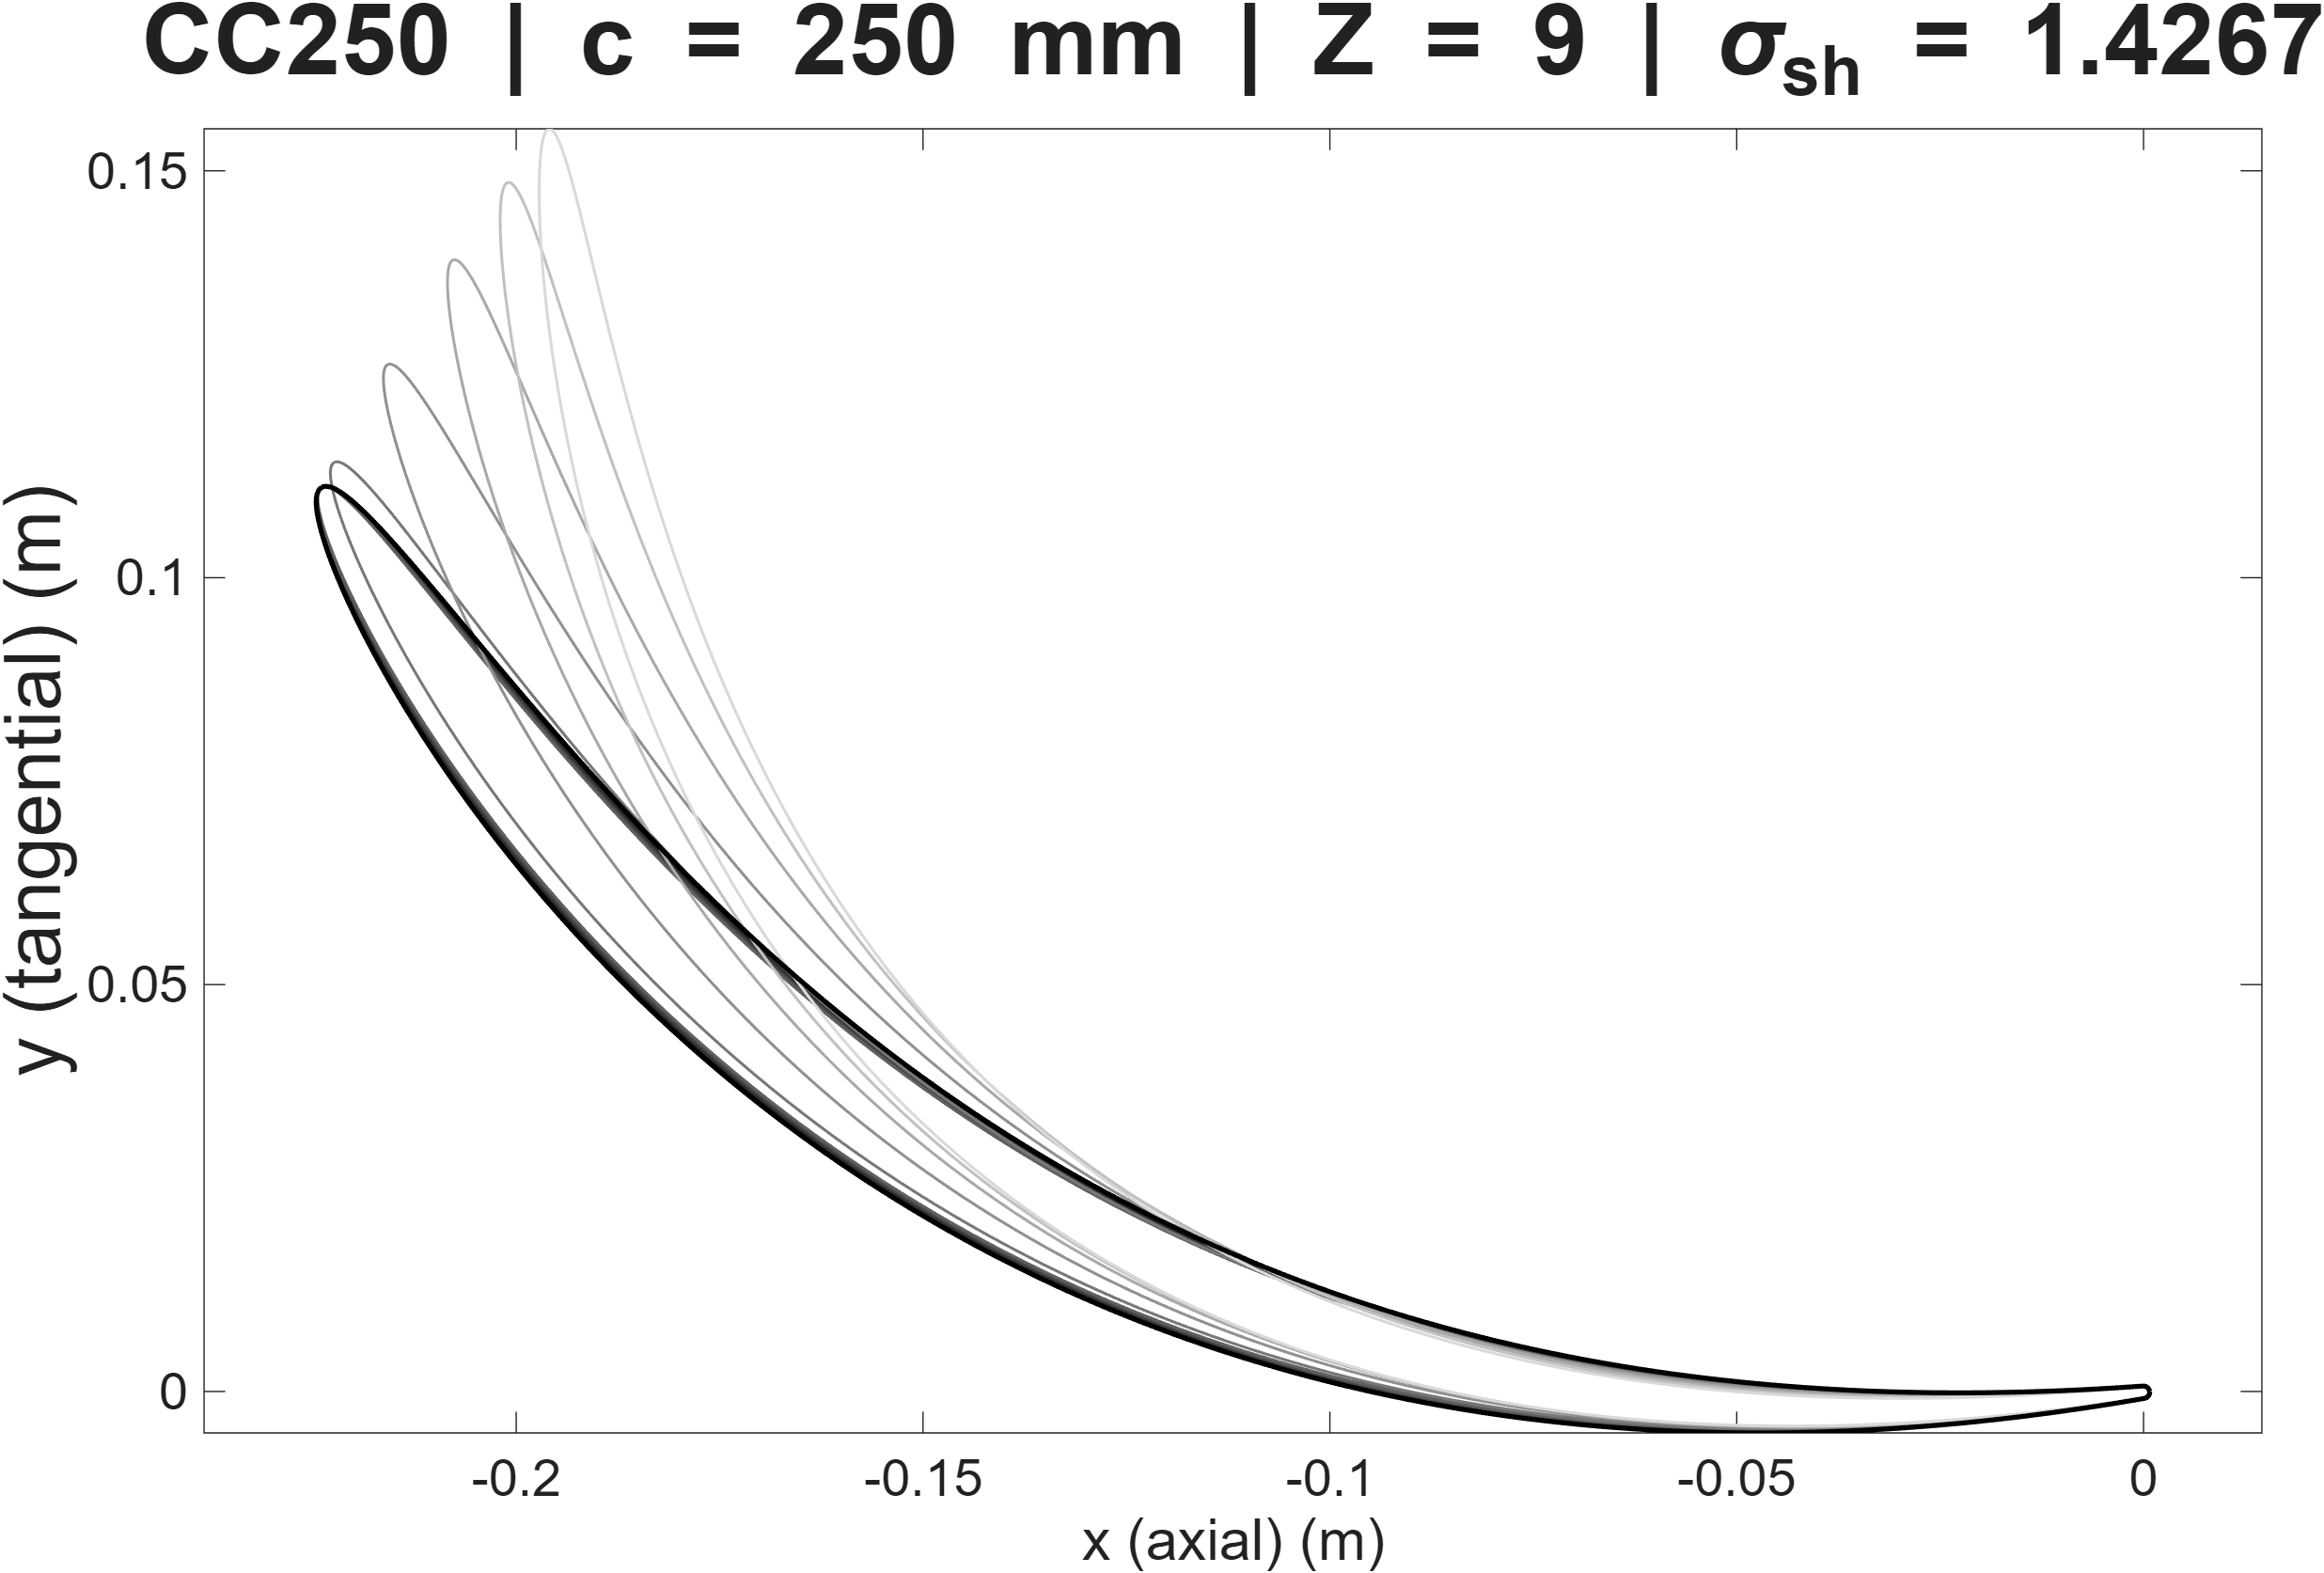
\includegraphics[width=\textwidth]{Figures/Foil2d/GV_Designs_2D/CC_250_9_2D.png}
    \caption{\texttt{CC\_250\_9}: $c = 250$~mm, $Z_s = 9$, $\sigma_{\mathrm{shroud}} = 1.43$.}
  \end{subfigure}
  \hfill
  \begin{subfigure}[b]{0.48\textwidth}
    \centering
    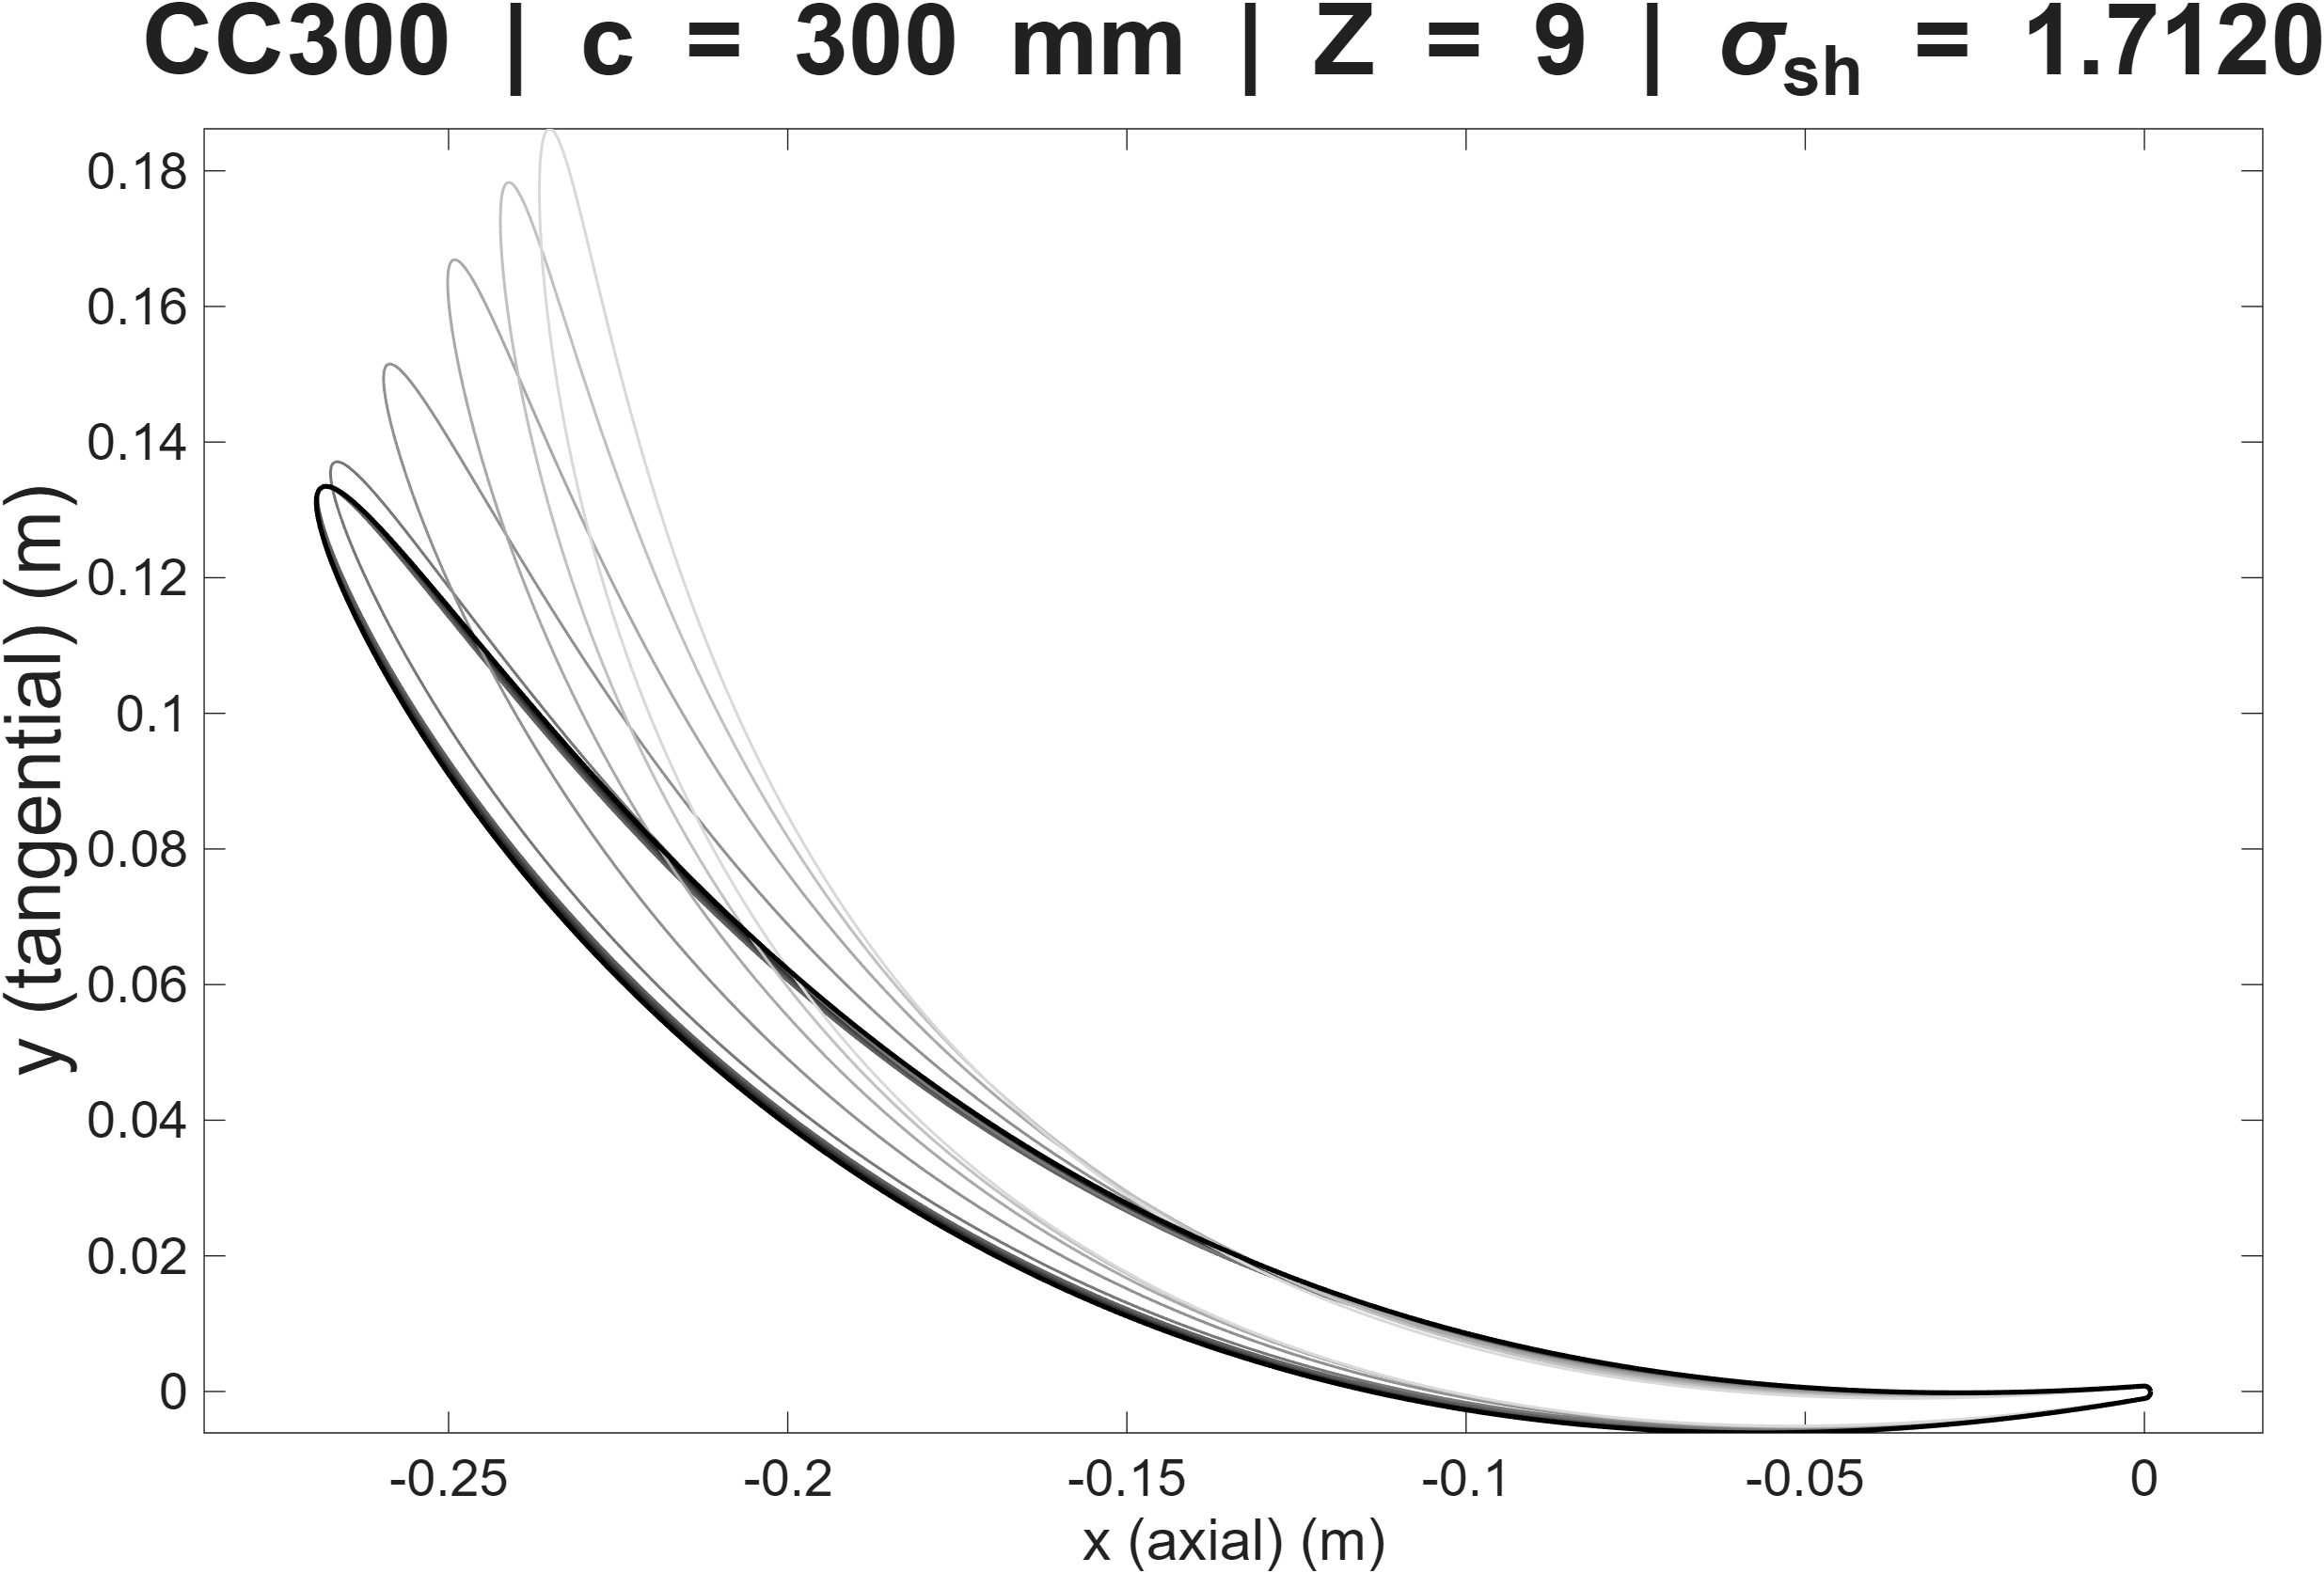
\includegraphics[width=\textwidth]{Figures/Foil2d/GV_Designs_2D/CC_300_9_2D.png}
    \caption{\texttt{CC\_300\_9}: $c = 300$~mm, $Z_s = 9$, $\sigma_{\mathrm{shroud}} = 1.71$.}
  \end{subfigure}

  \vspace{0.6em}

  \begin{subfigure}[b]{0.48\textwidth}
    \centering
    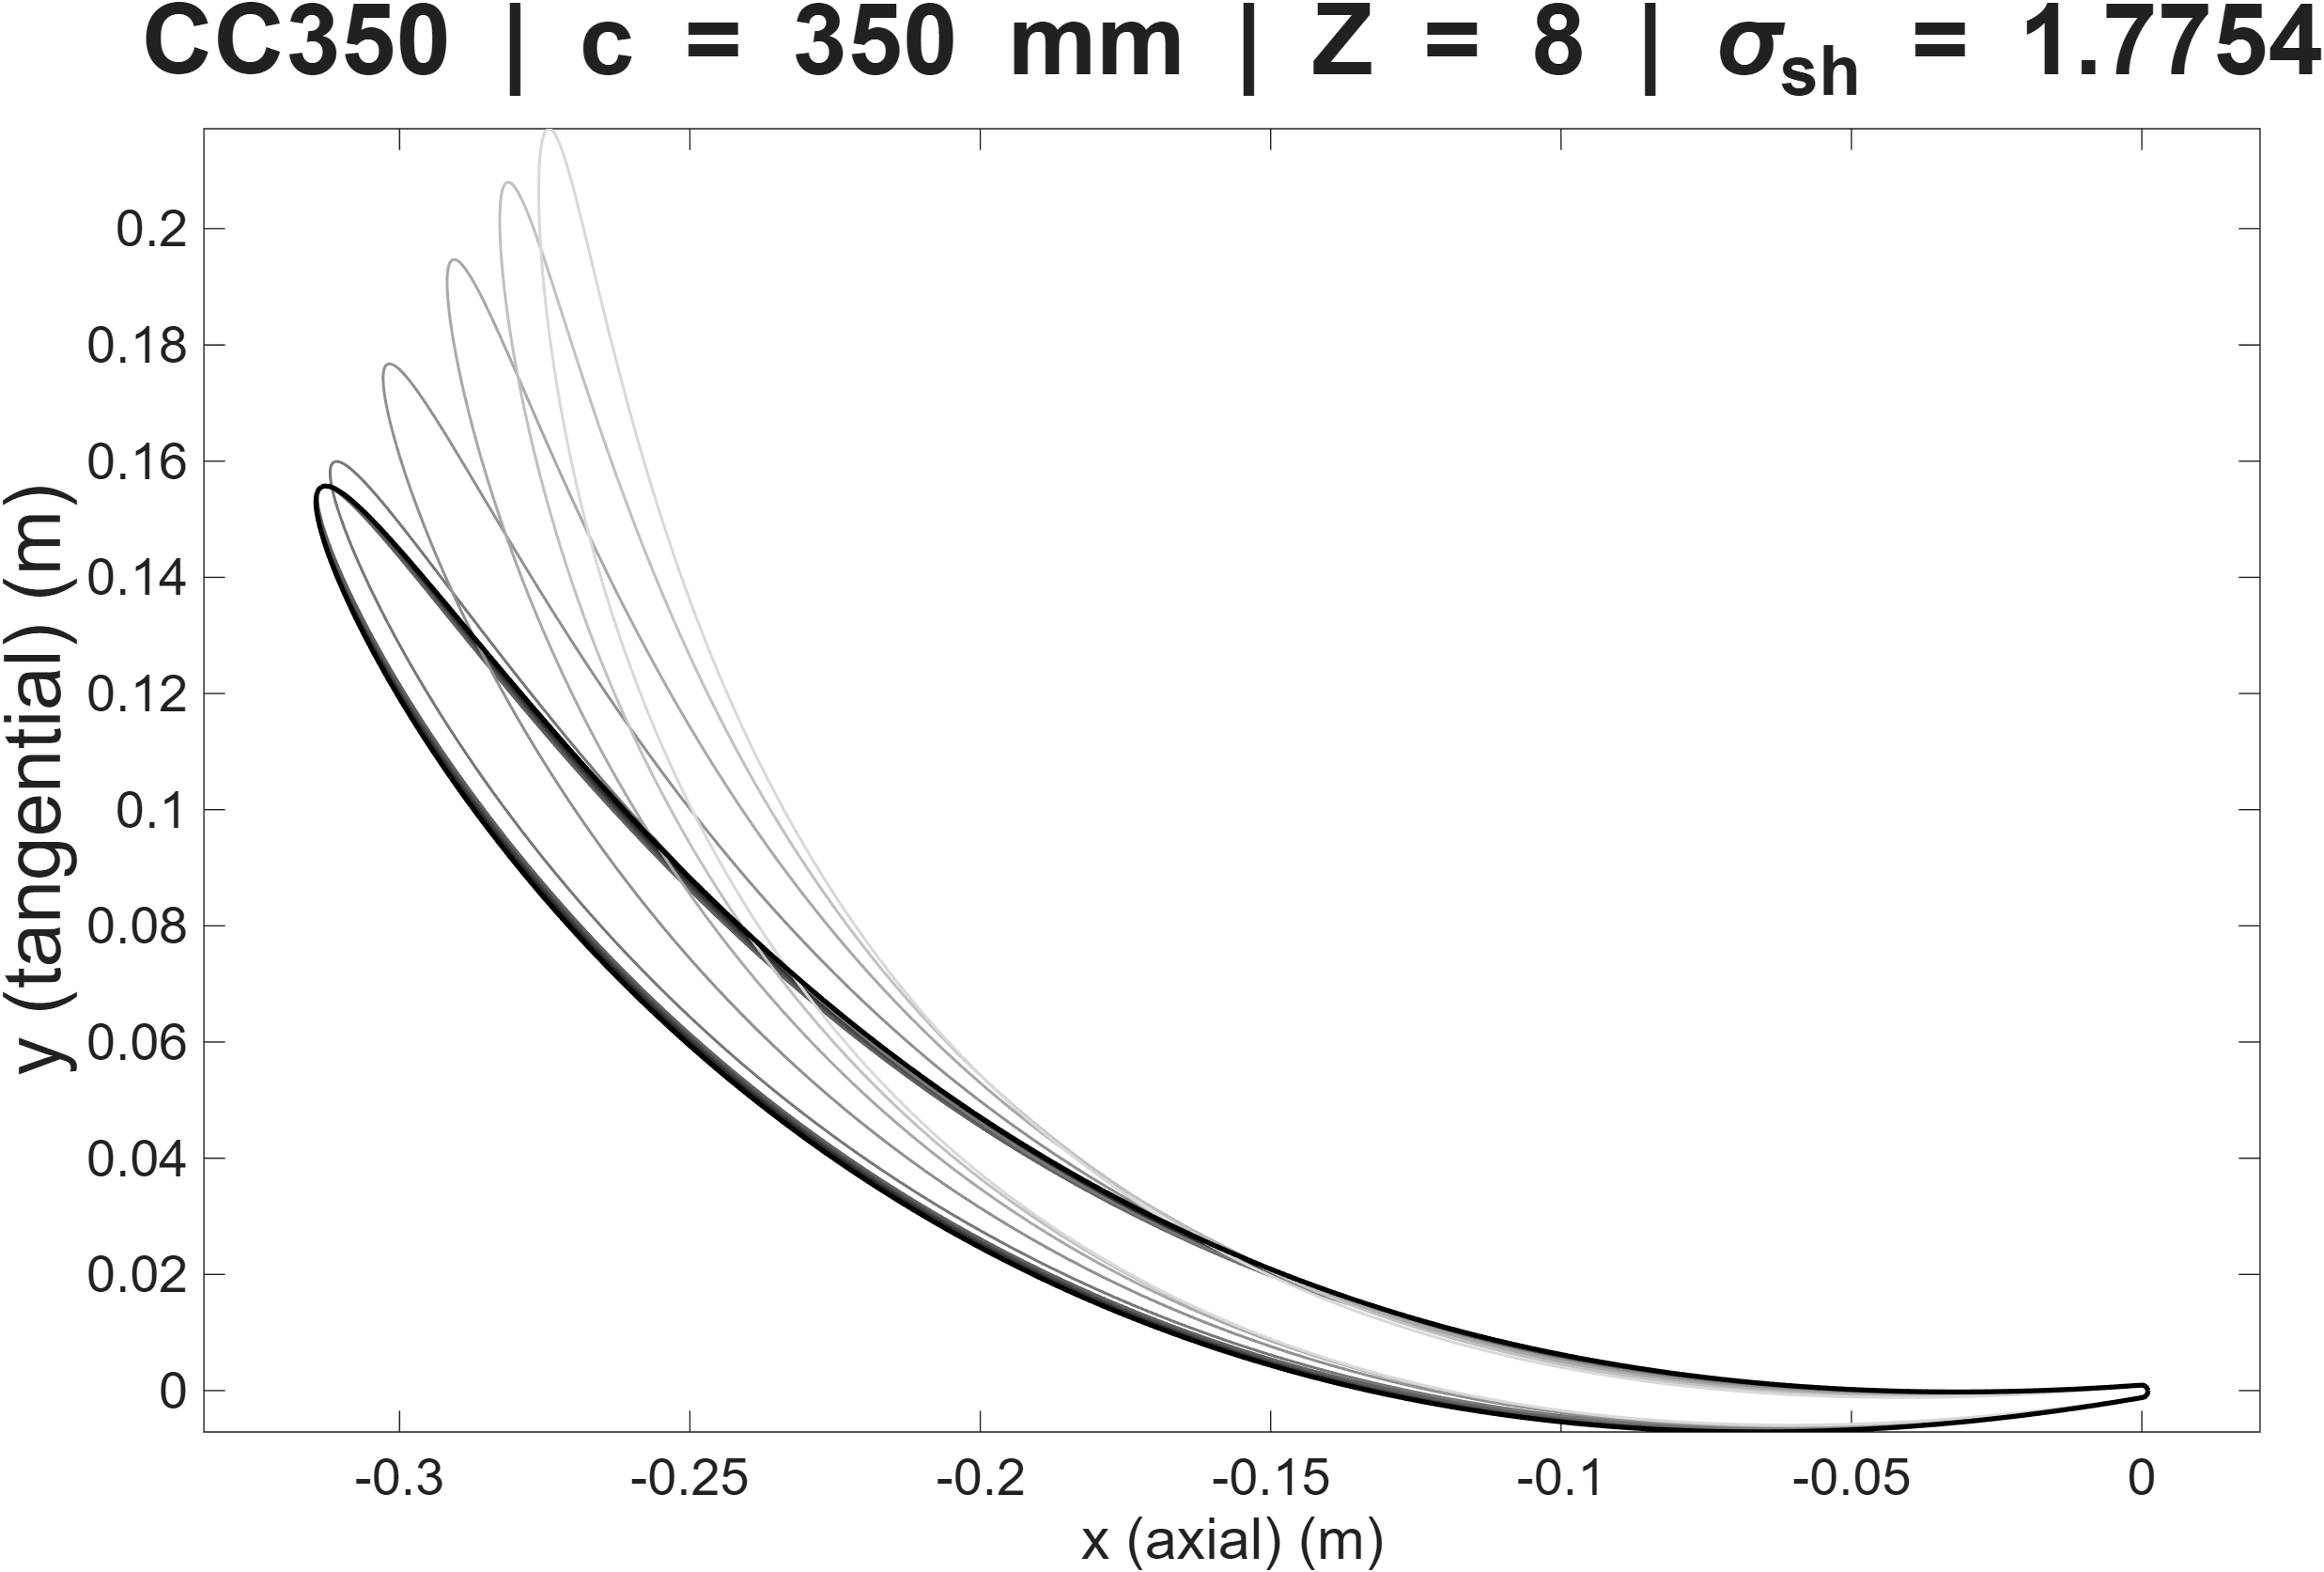
\includegraphics[width=\textwidth]{Figures/Foil2d/GV_Designs_2D/CC_350_8_2D.png}
    \caption{\texttt{CC\_350\_8}: $c = 350$~mm, $Z_s = 8$, $\sigma_{\mathrm{shroud}} = 1.78$.}
  \end{subfigure}
  \hfill
  \begin{subfigure}[b]{0.48\textwidth}
    \centering
    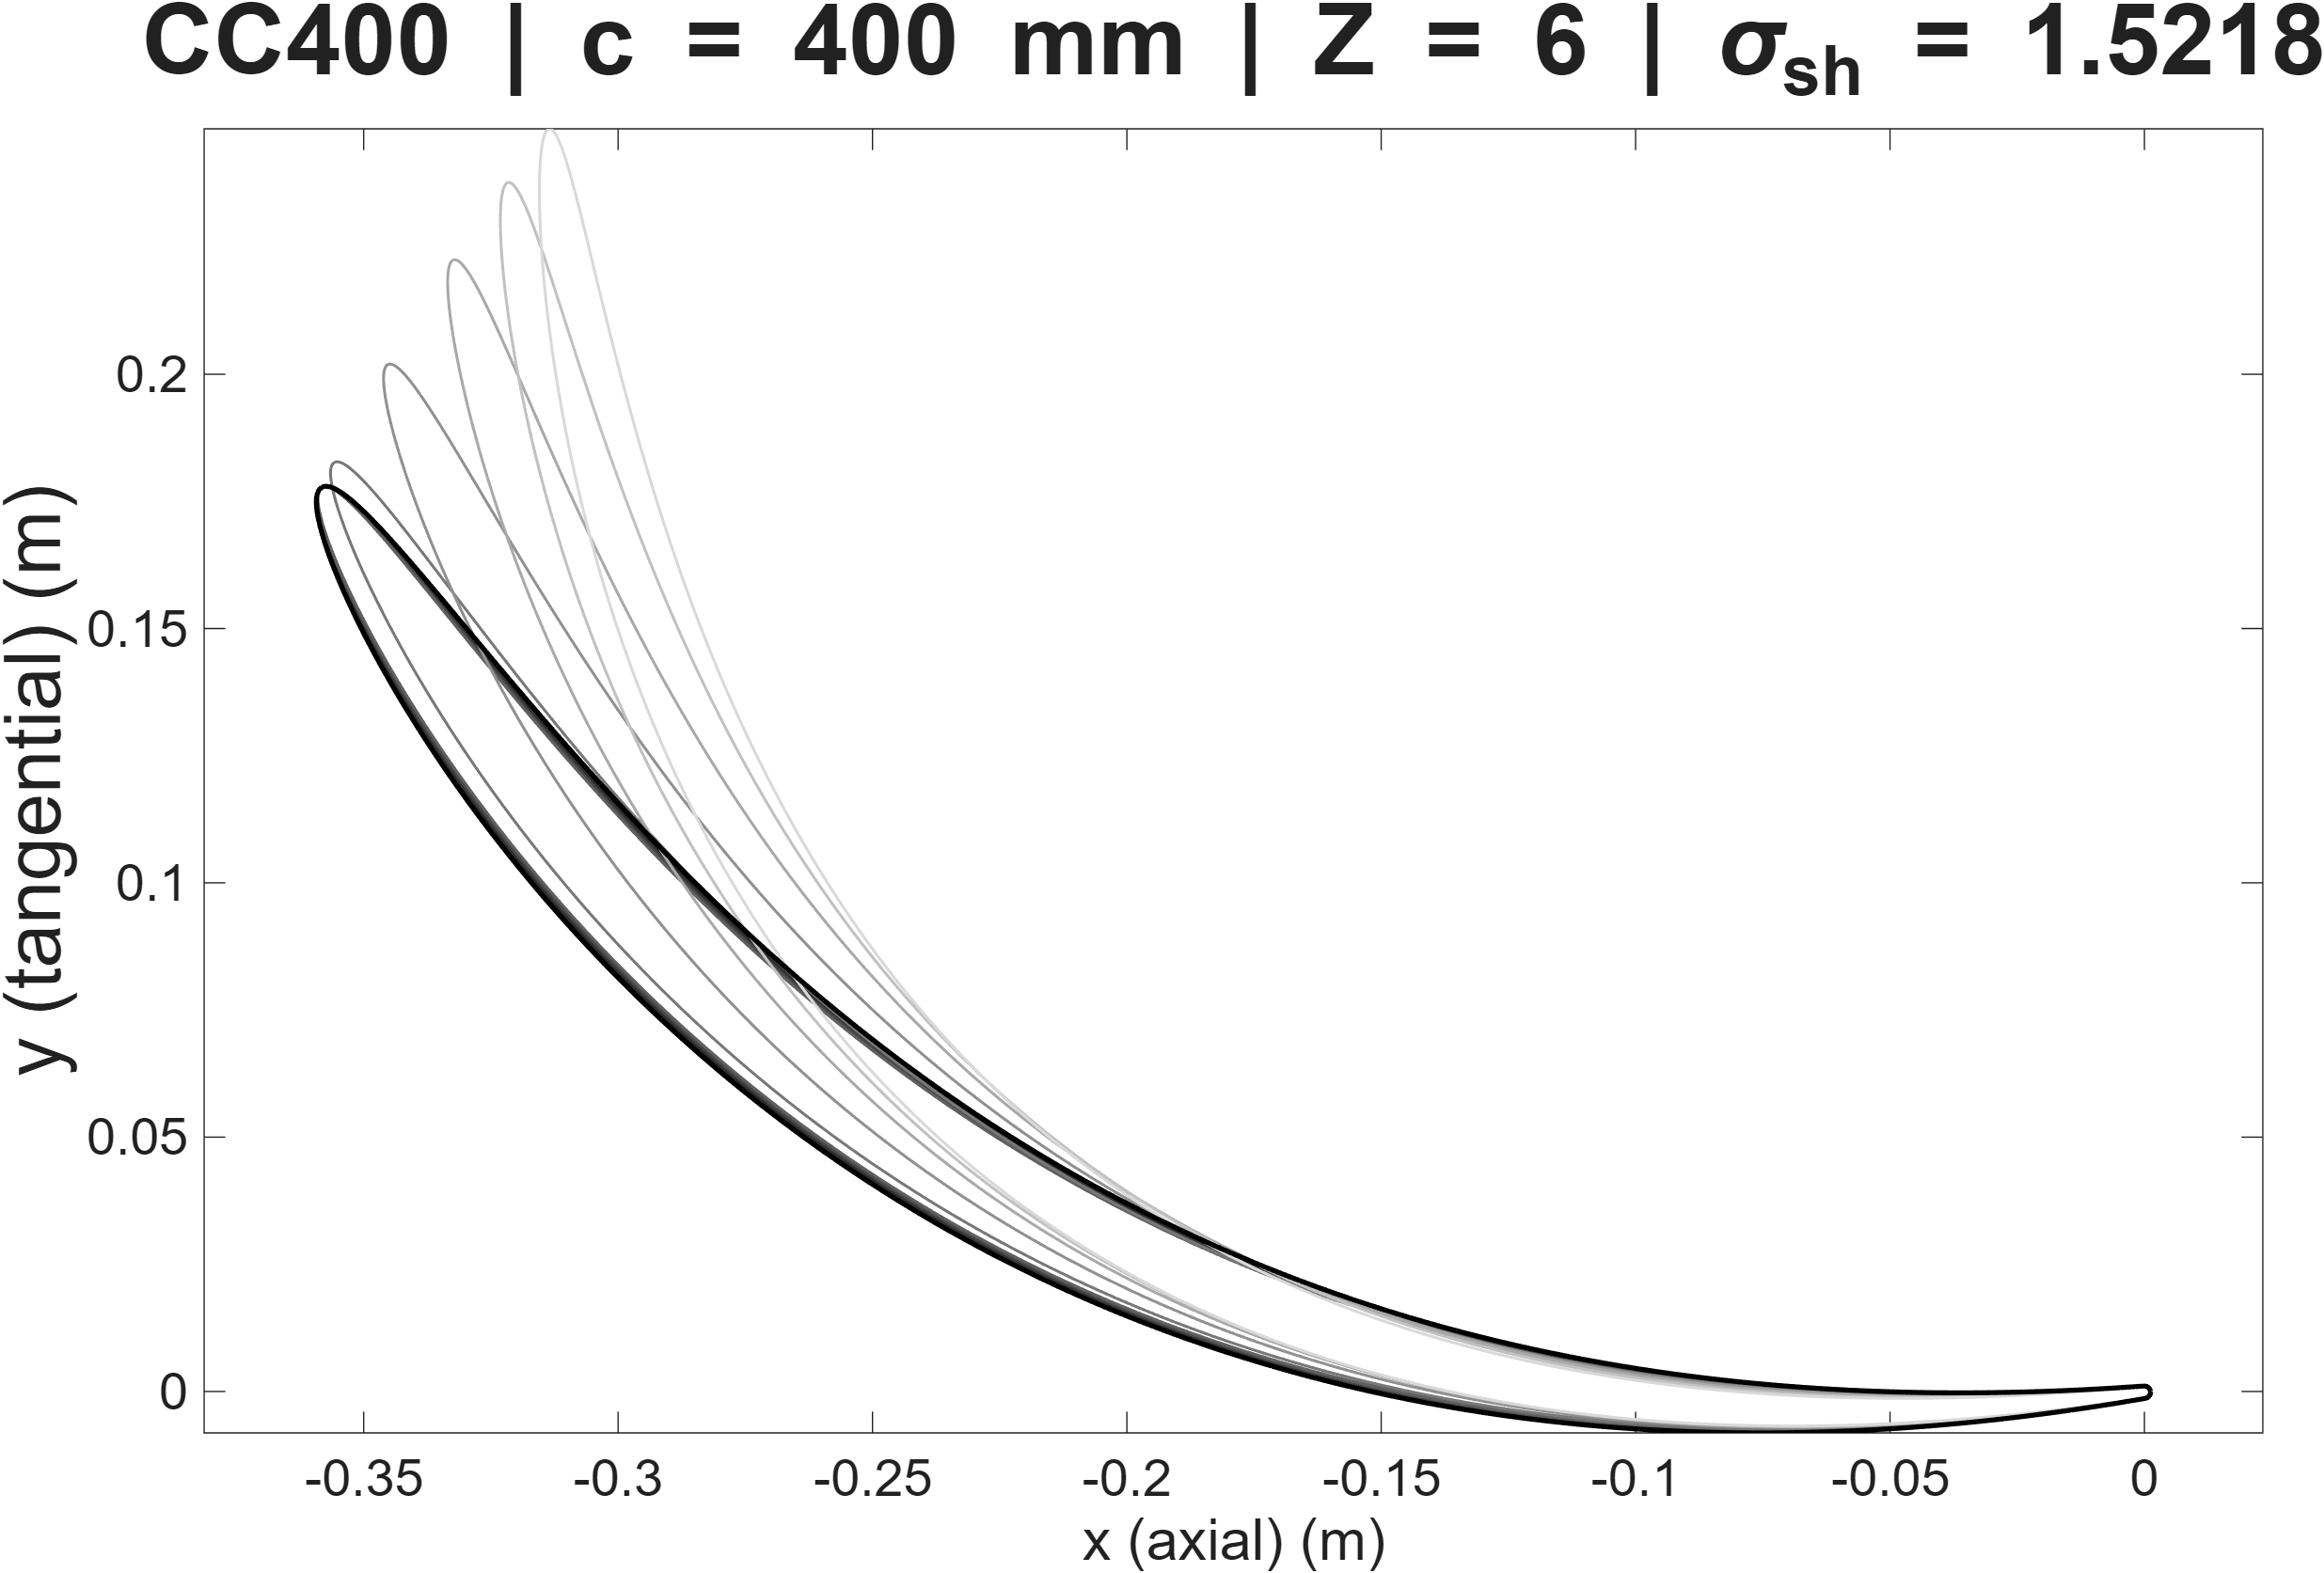
\includegraphics[width=\textwidth]{Figures/Foil2d/GV_Designs_2D/CC_400_6_2D.png}
    \caption{\texttt{CC\_400\_6}: $c = 400$~mm, $Z_s = 6$, $\sigma_{\mathrm{shroud}} = 1.52$.}
  \end{subfigure}

  \vspace{0.6em}

  \begin{subfigure}[b]{0.48\textwidth}
    \centering
    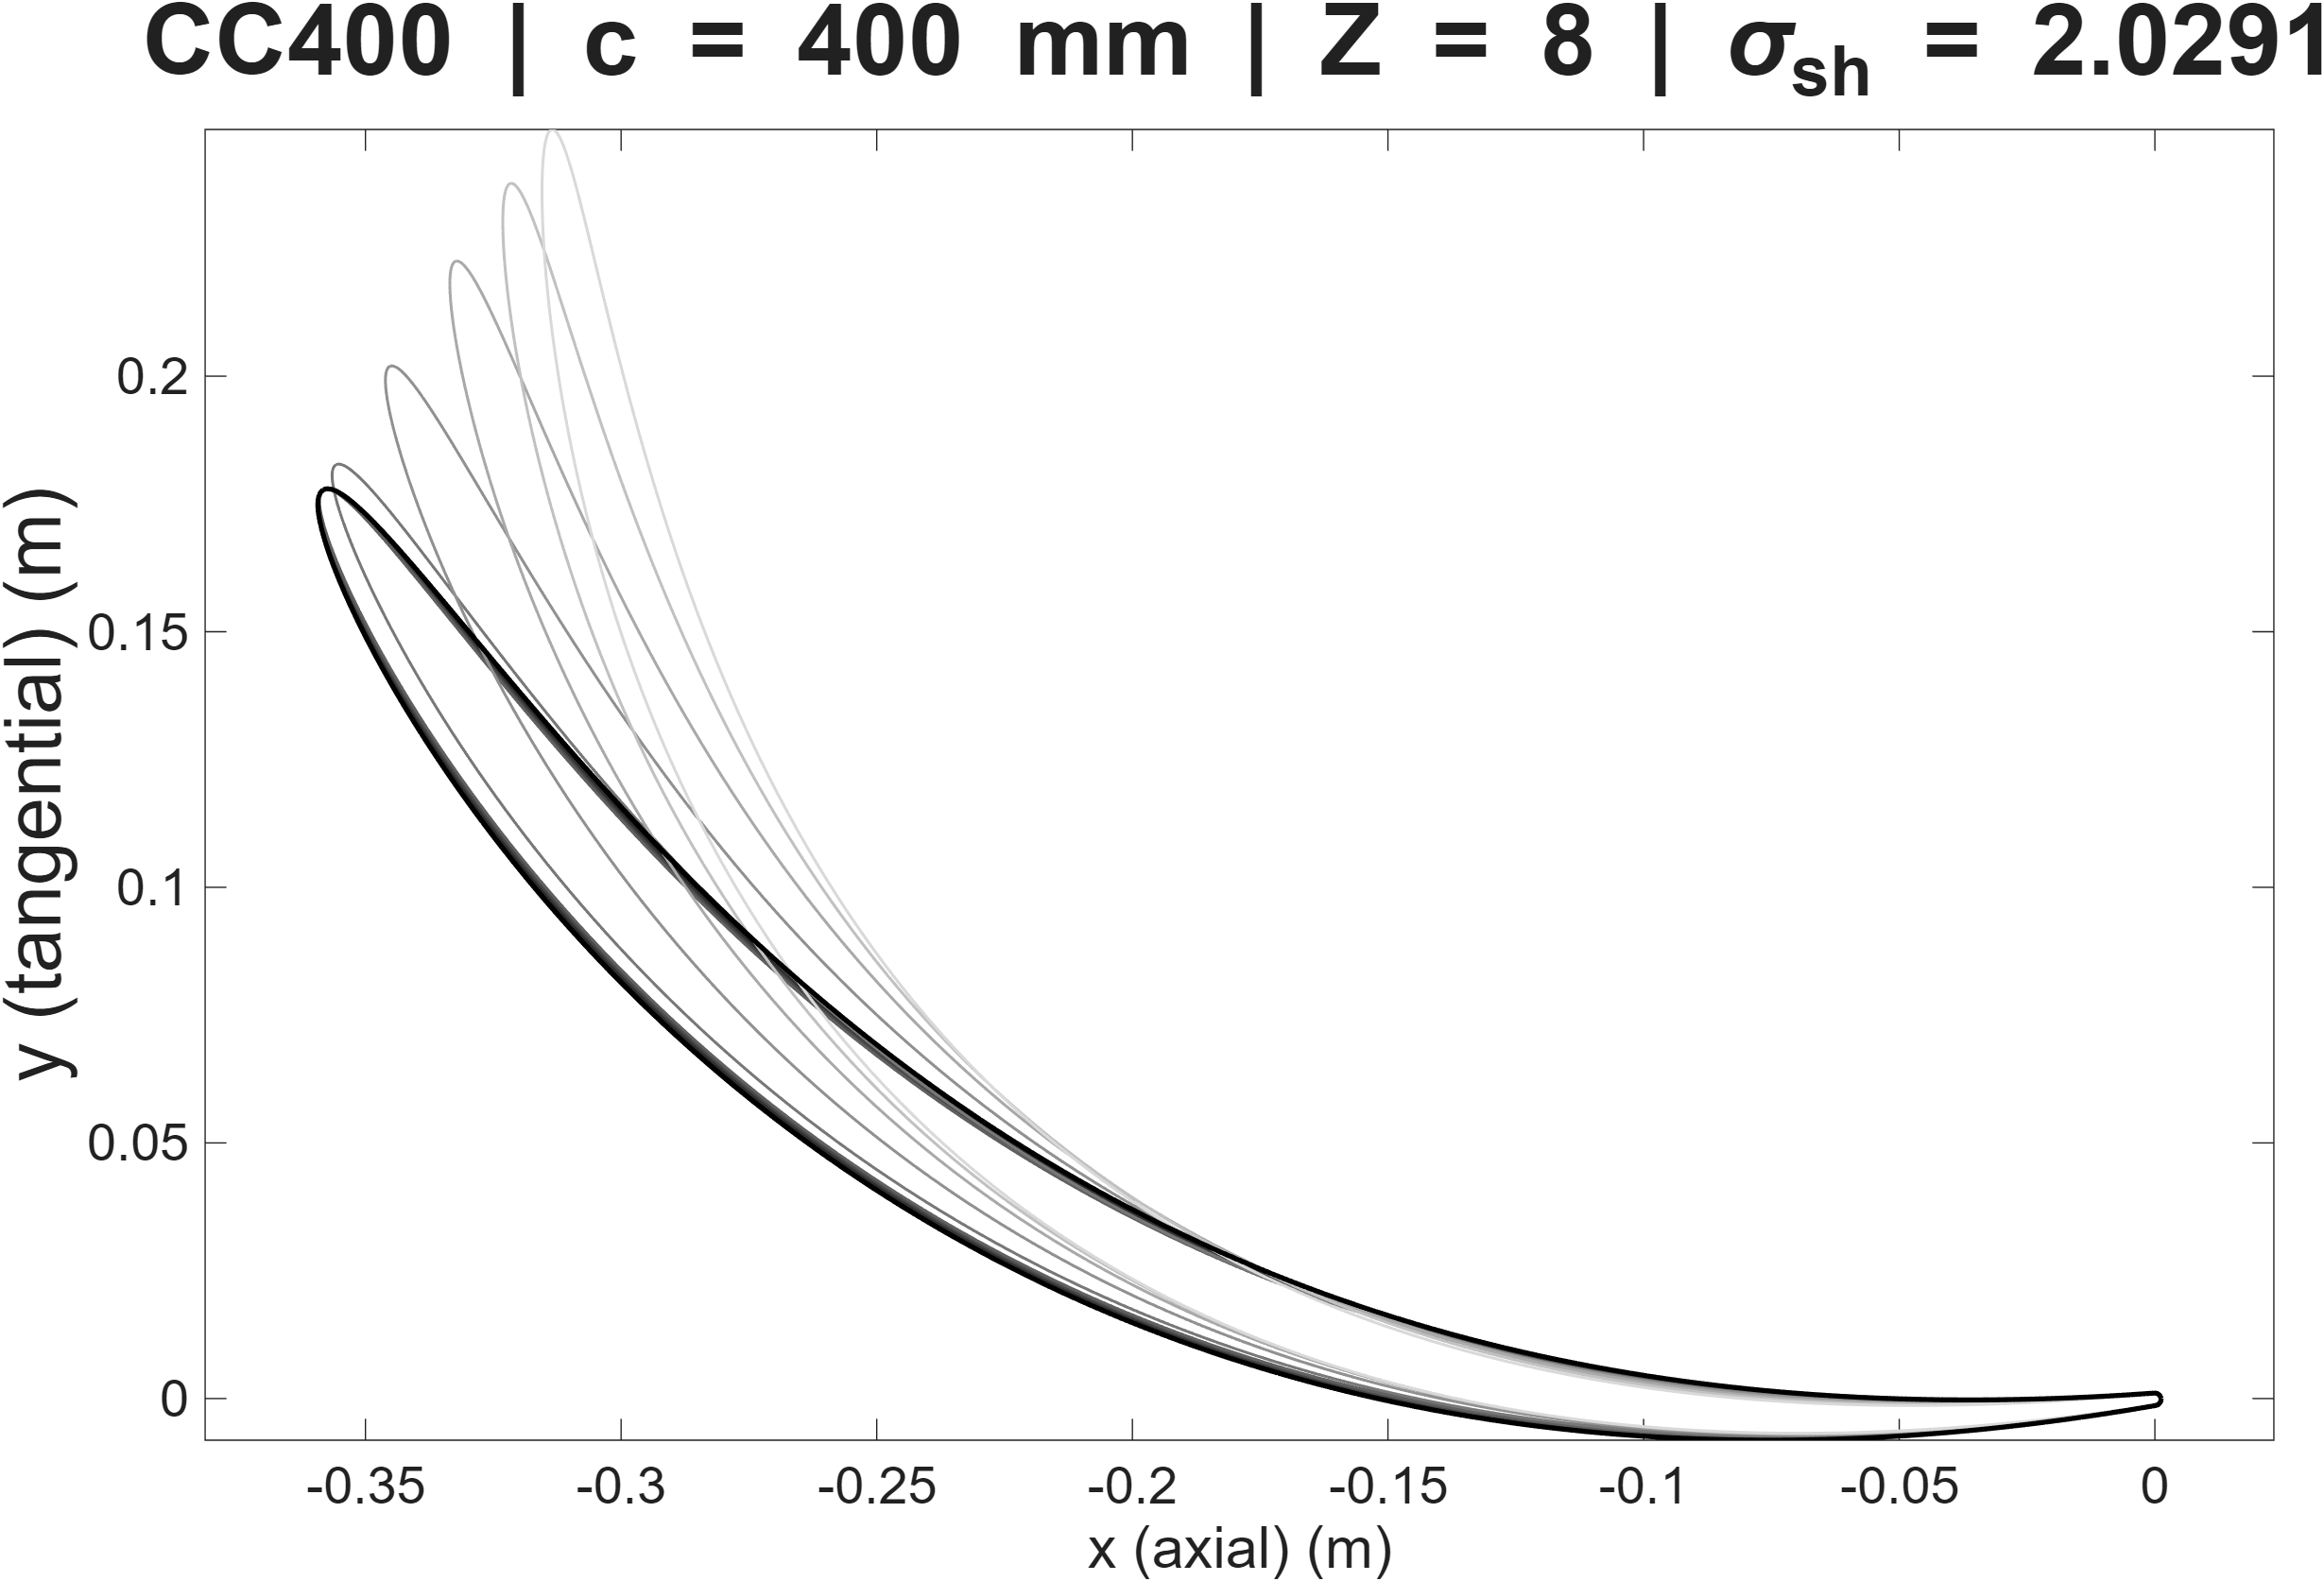
\includegraphics[width=\textwidth]{Figures/Foil2d/GV_Designs_2D/CC_400_8_2D.png}
    \caption{\texttt{CC\_400\_8}: $c = 400$~mm, $Z_s = 8$, $\sigma_{\mathrm{shroud}} = 2.03$.}
  \end{subfigure}
  \hfill
  \begin{subfigure}[b]{0.48\textwidth}
    \centering
    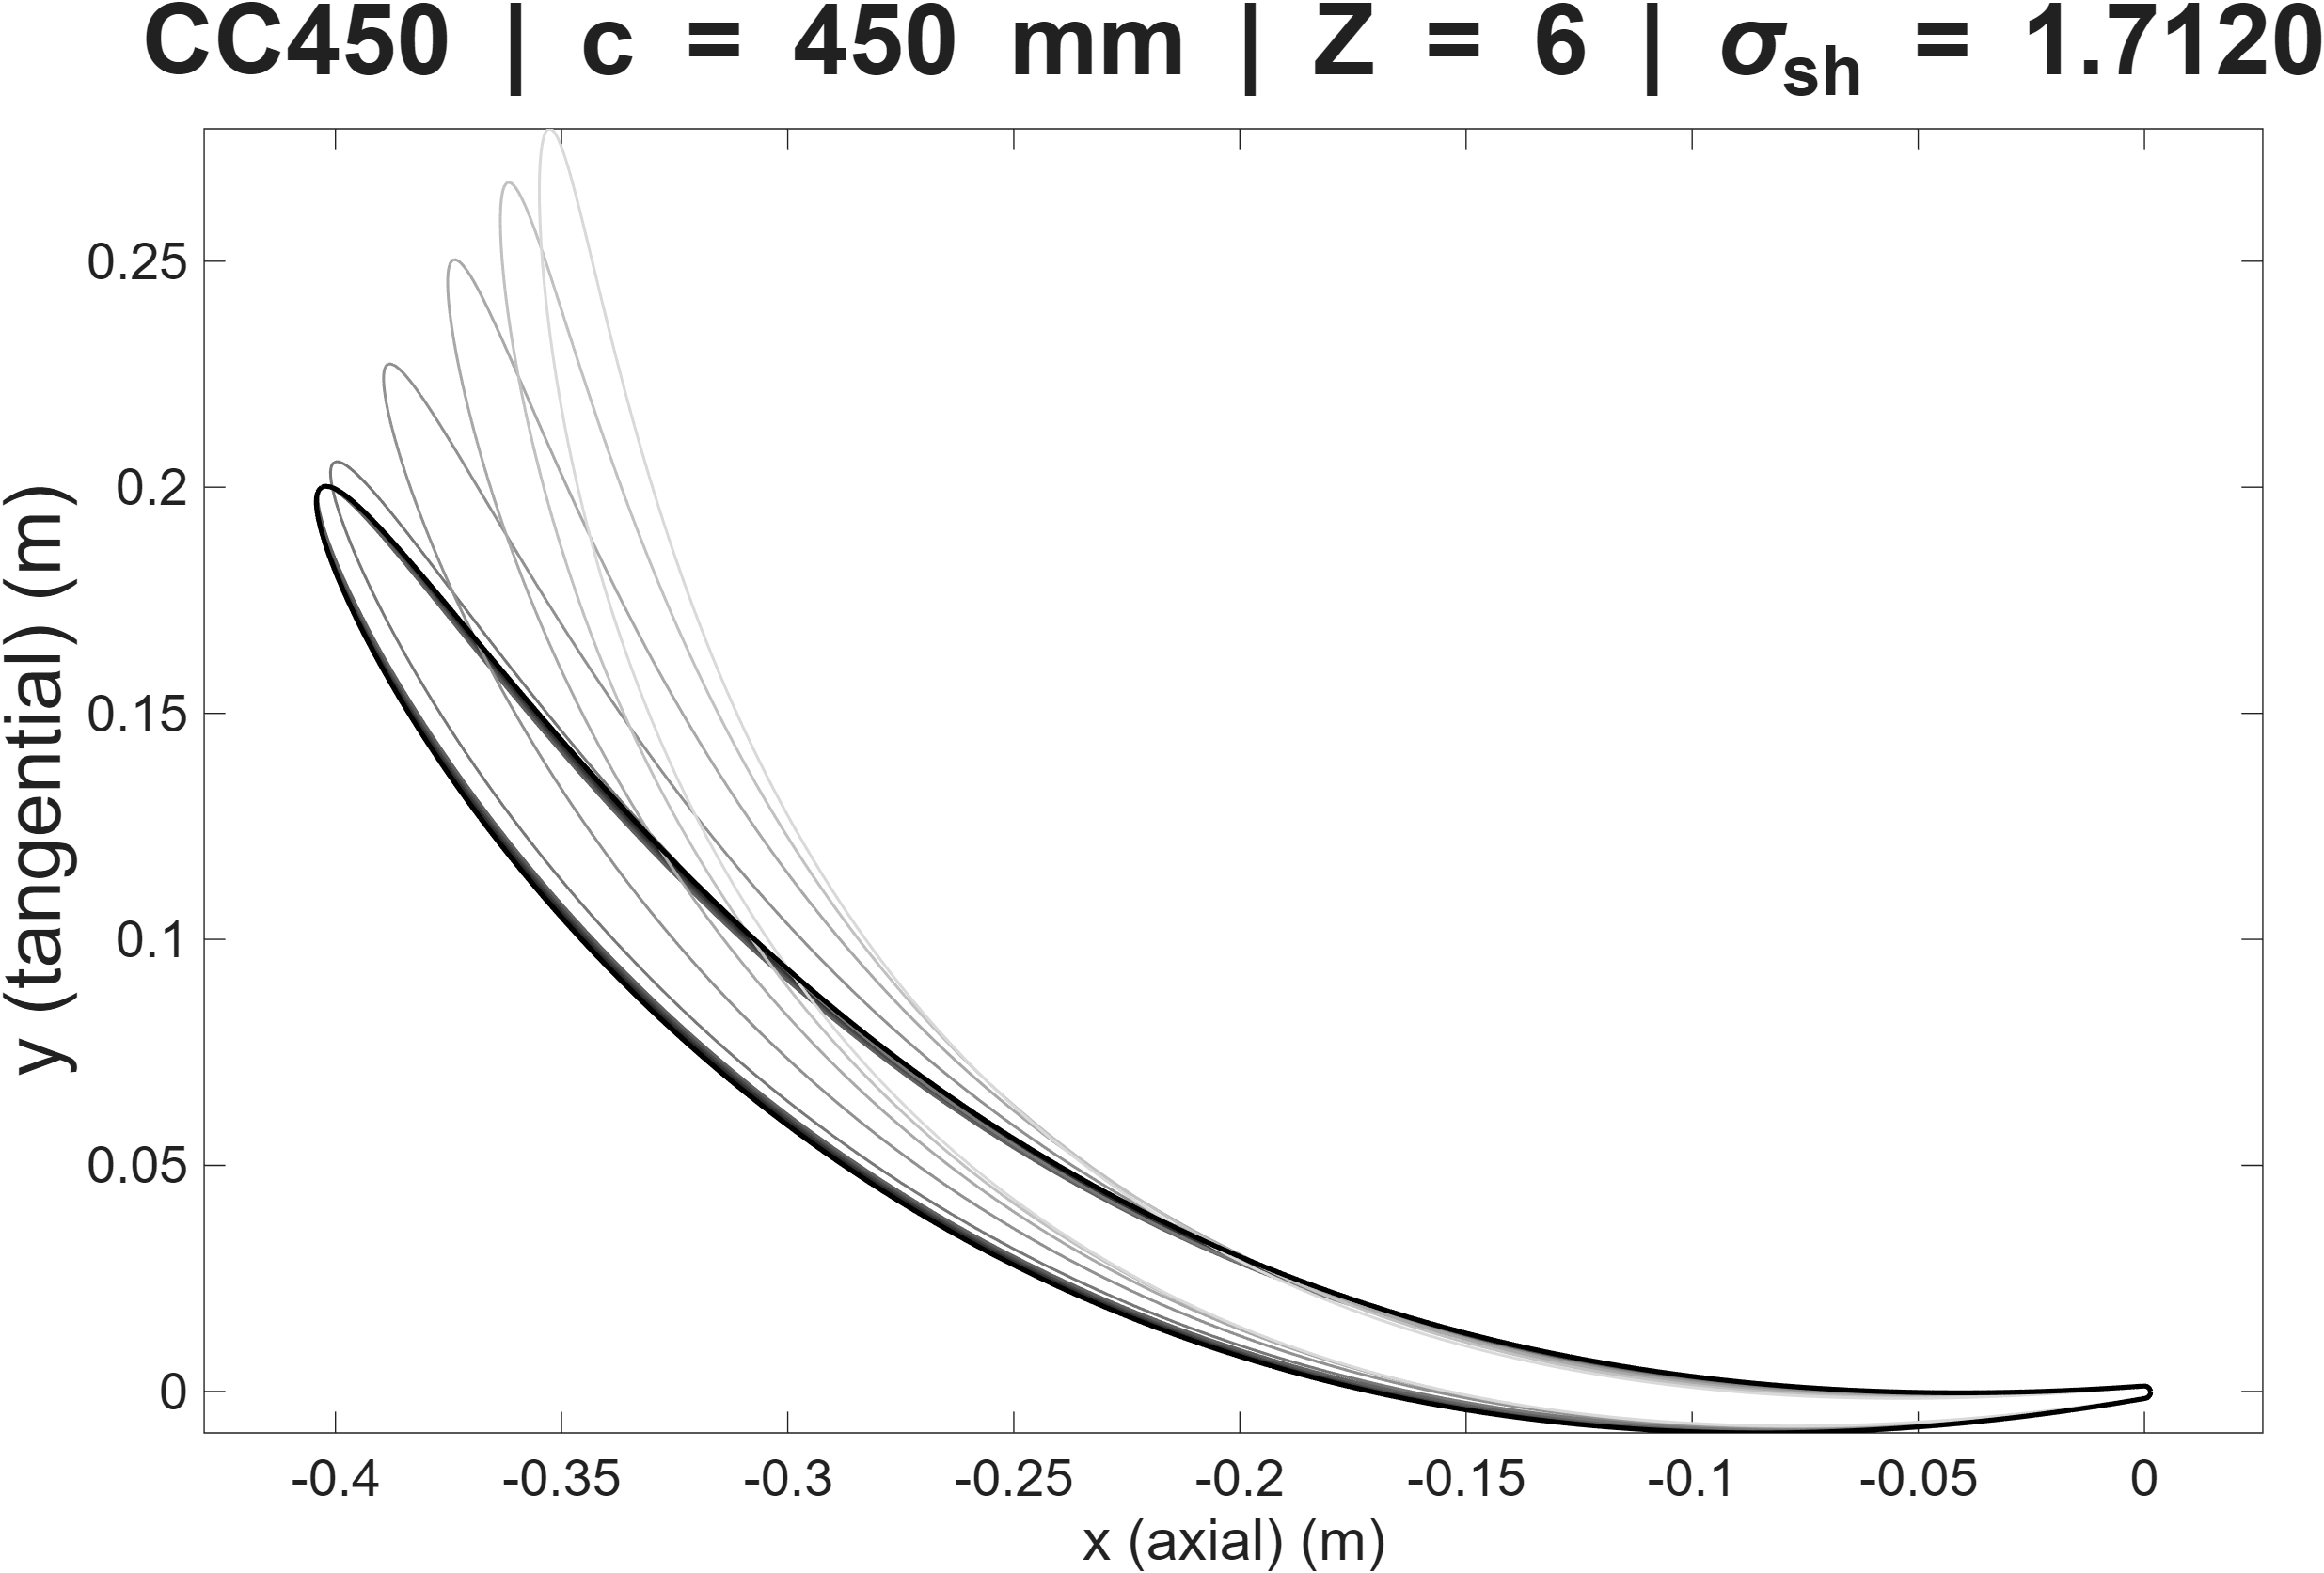
\includegraphics[width=\textwidth]{Figures/Foil2d/GV_Designs_2D/CC_450_6_2D.png}
    \caption{\texttt{CC\_450\_6}: $c = 450$~mm, $Z_s = 6$, $\sigma_{\mathrm{shroud}} = 1.71$.}
  \end{subfigure}

  \caption[CC family 2D sections, part 1 of 2]{Two-dimensional section stacks of the constant-chord (CC) family, configurations \texttt{CC\_250\_9} through \texttt{CC\_450\_6}. The chord is identical at every radius, so the section outlines overlap closely along the span.}
  \label{fig:cc_2d_1}
\end{figure}

\begin{figure}[H]
  \centering
  \begin{subfigure}[b]{0.48\textwidth}
    \centering
    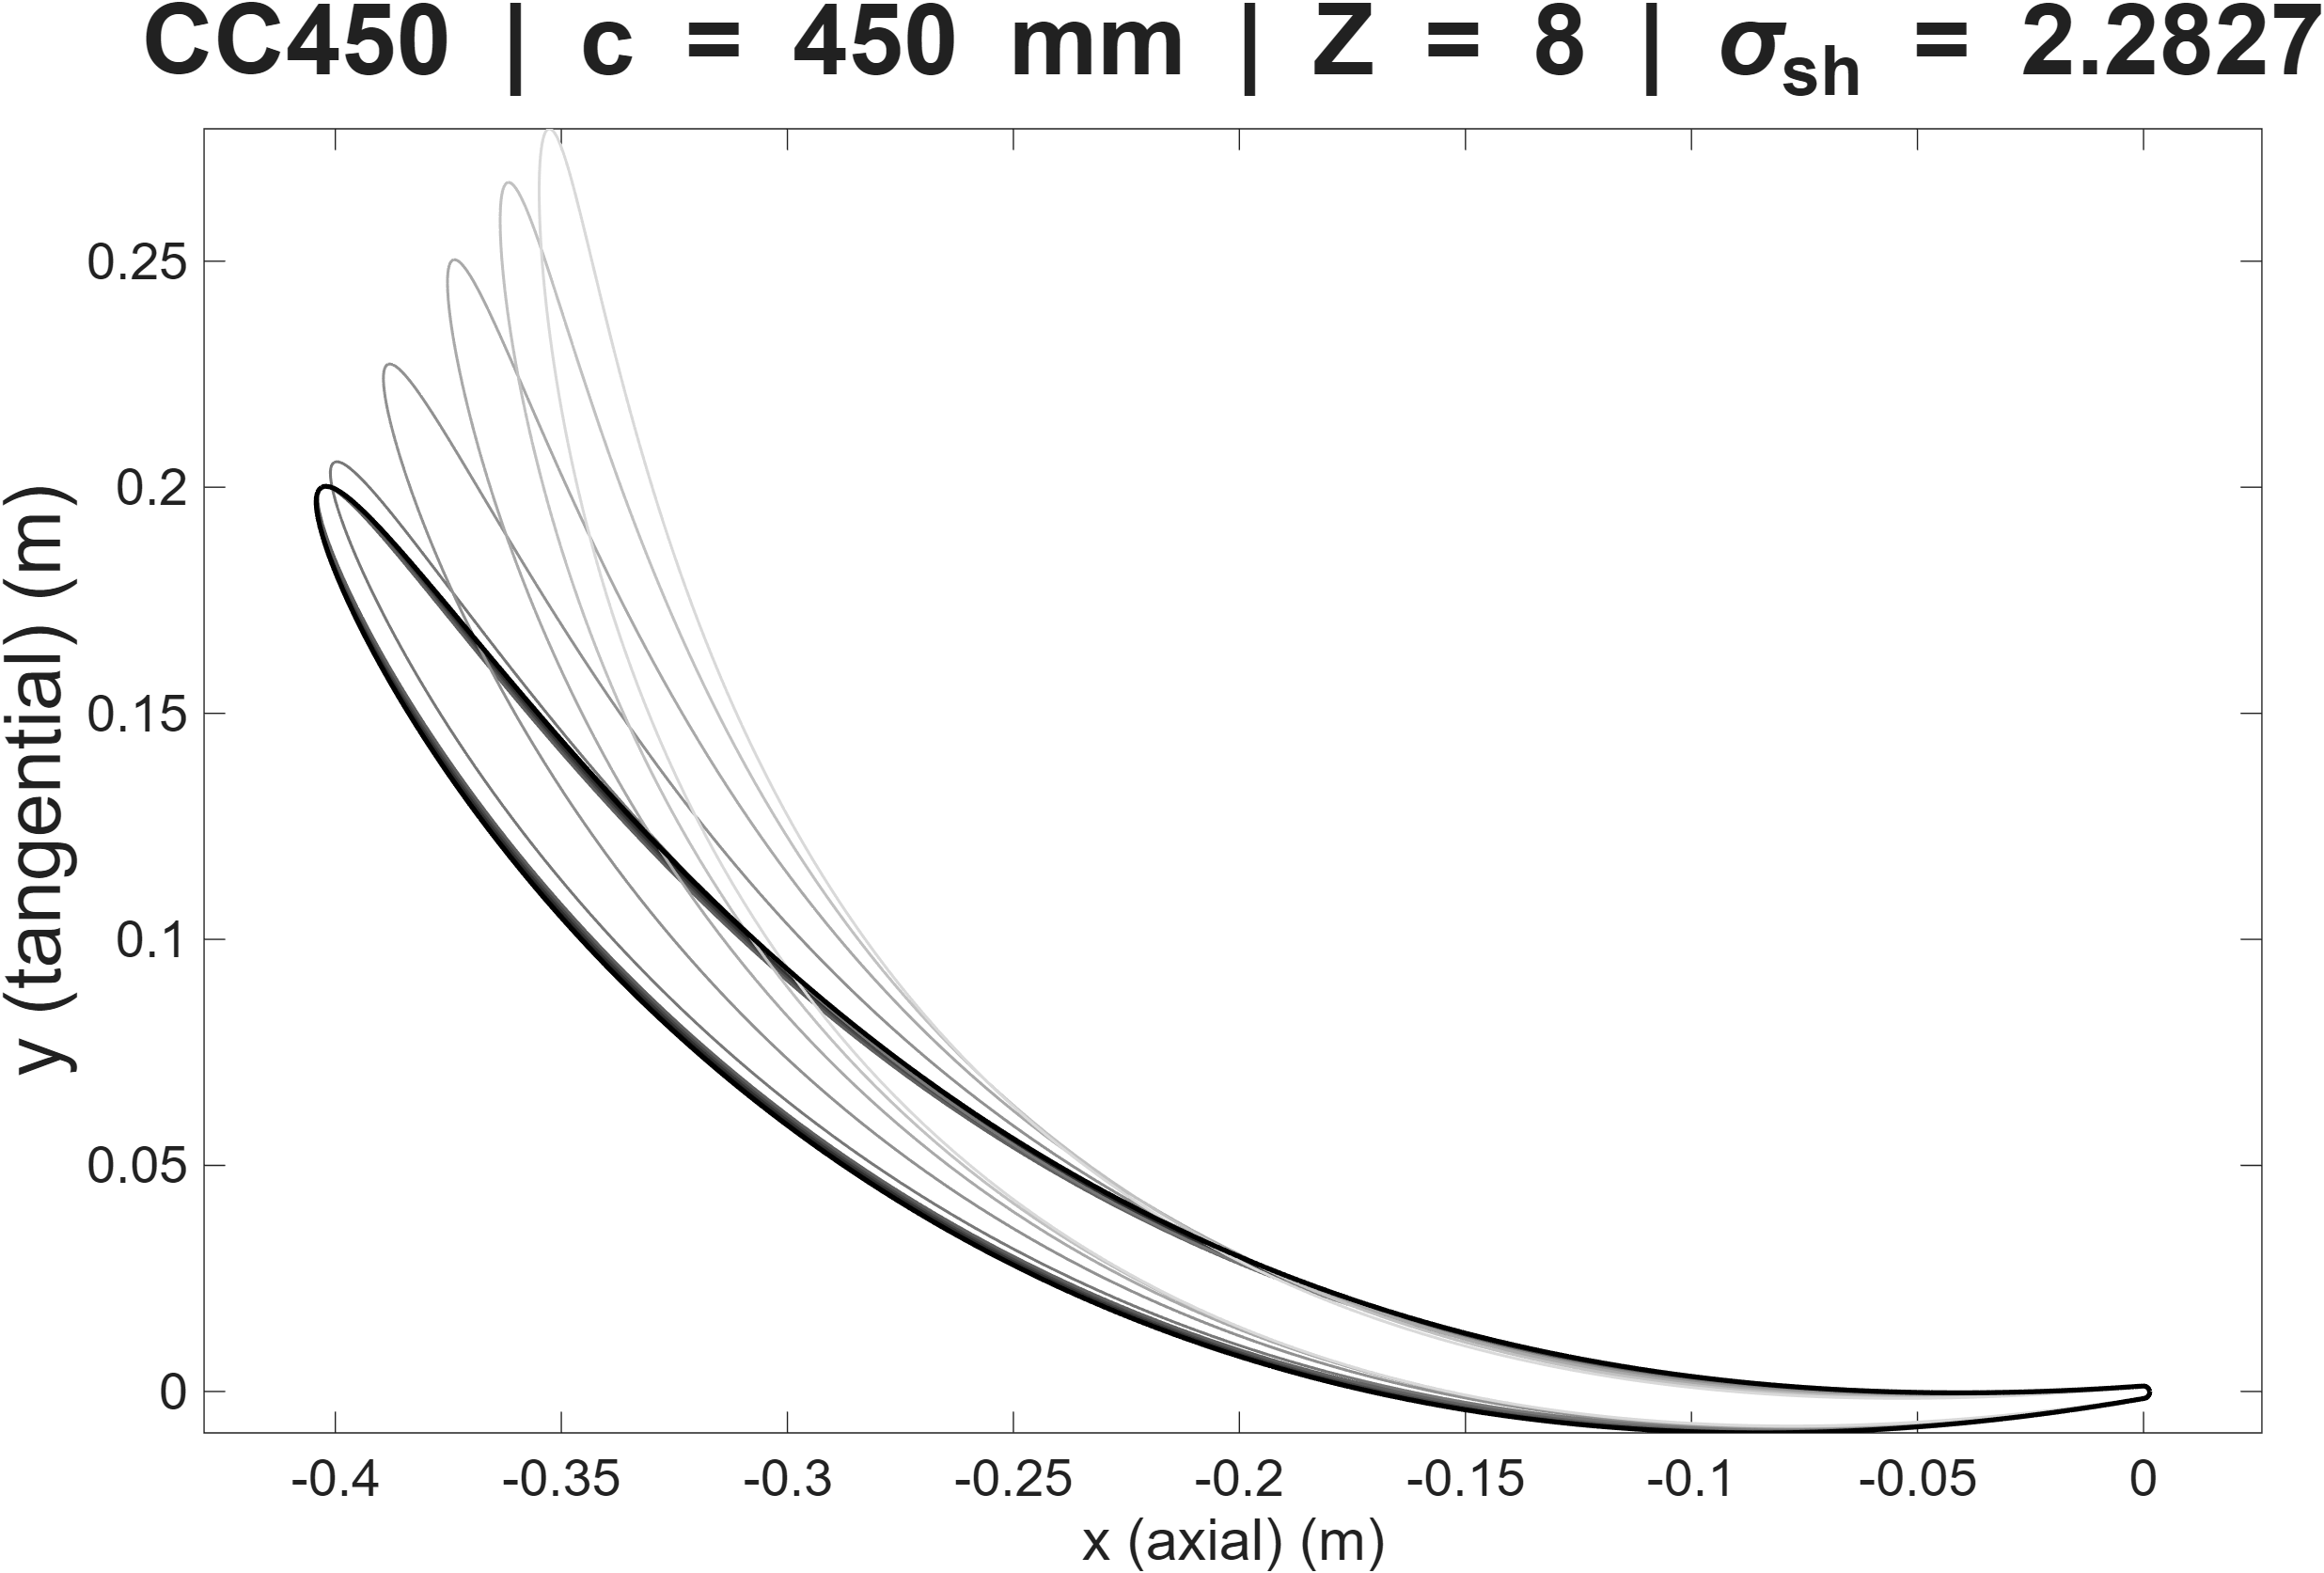
\includegraphics[width=\textwidth]{Figures/Foil2d/GV_Designs_2D/CC_450_8_2D.png}
    \caption{\texttt{CC\_450\_8}: $c = 450$~mm, $Z_s = 8$, $\sigma_{\mathrm{shroud}} = 2.28$.}
  \end{subfigure}
  \hfill
  \begin{subfigure}[b]{0.48\textwidth}
    \centering
    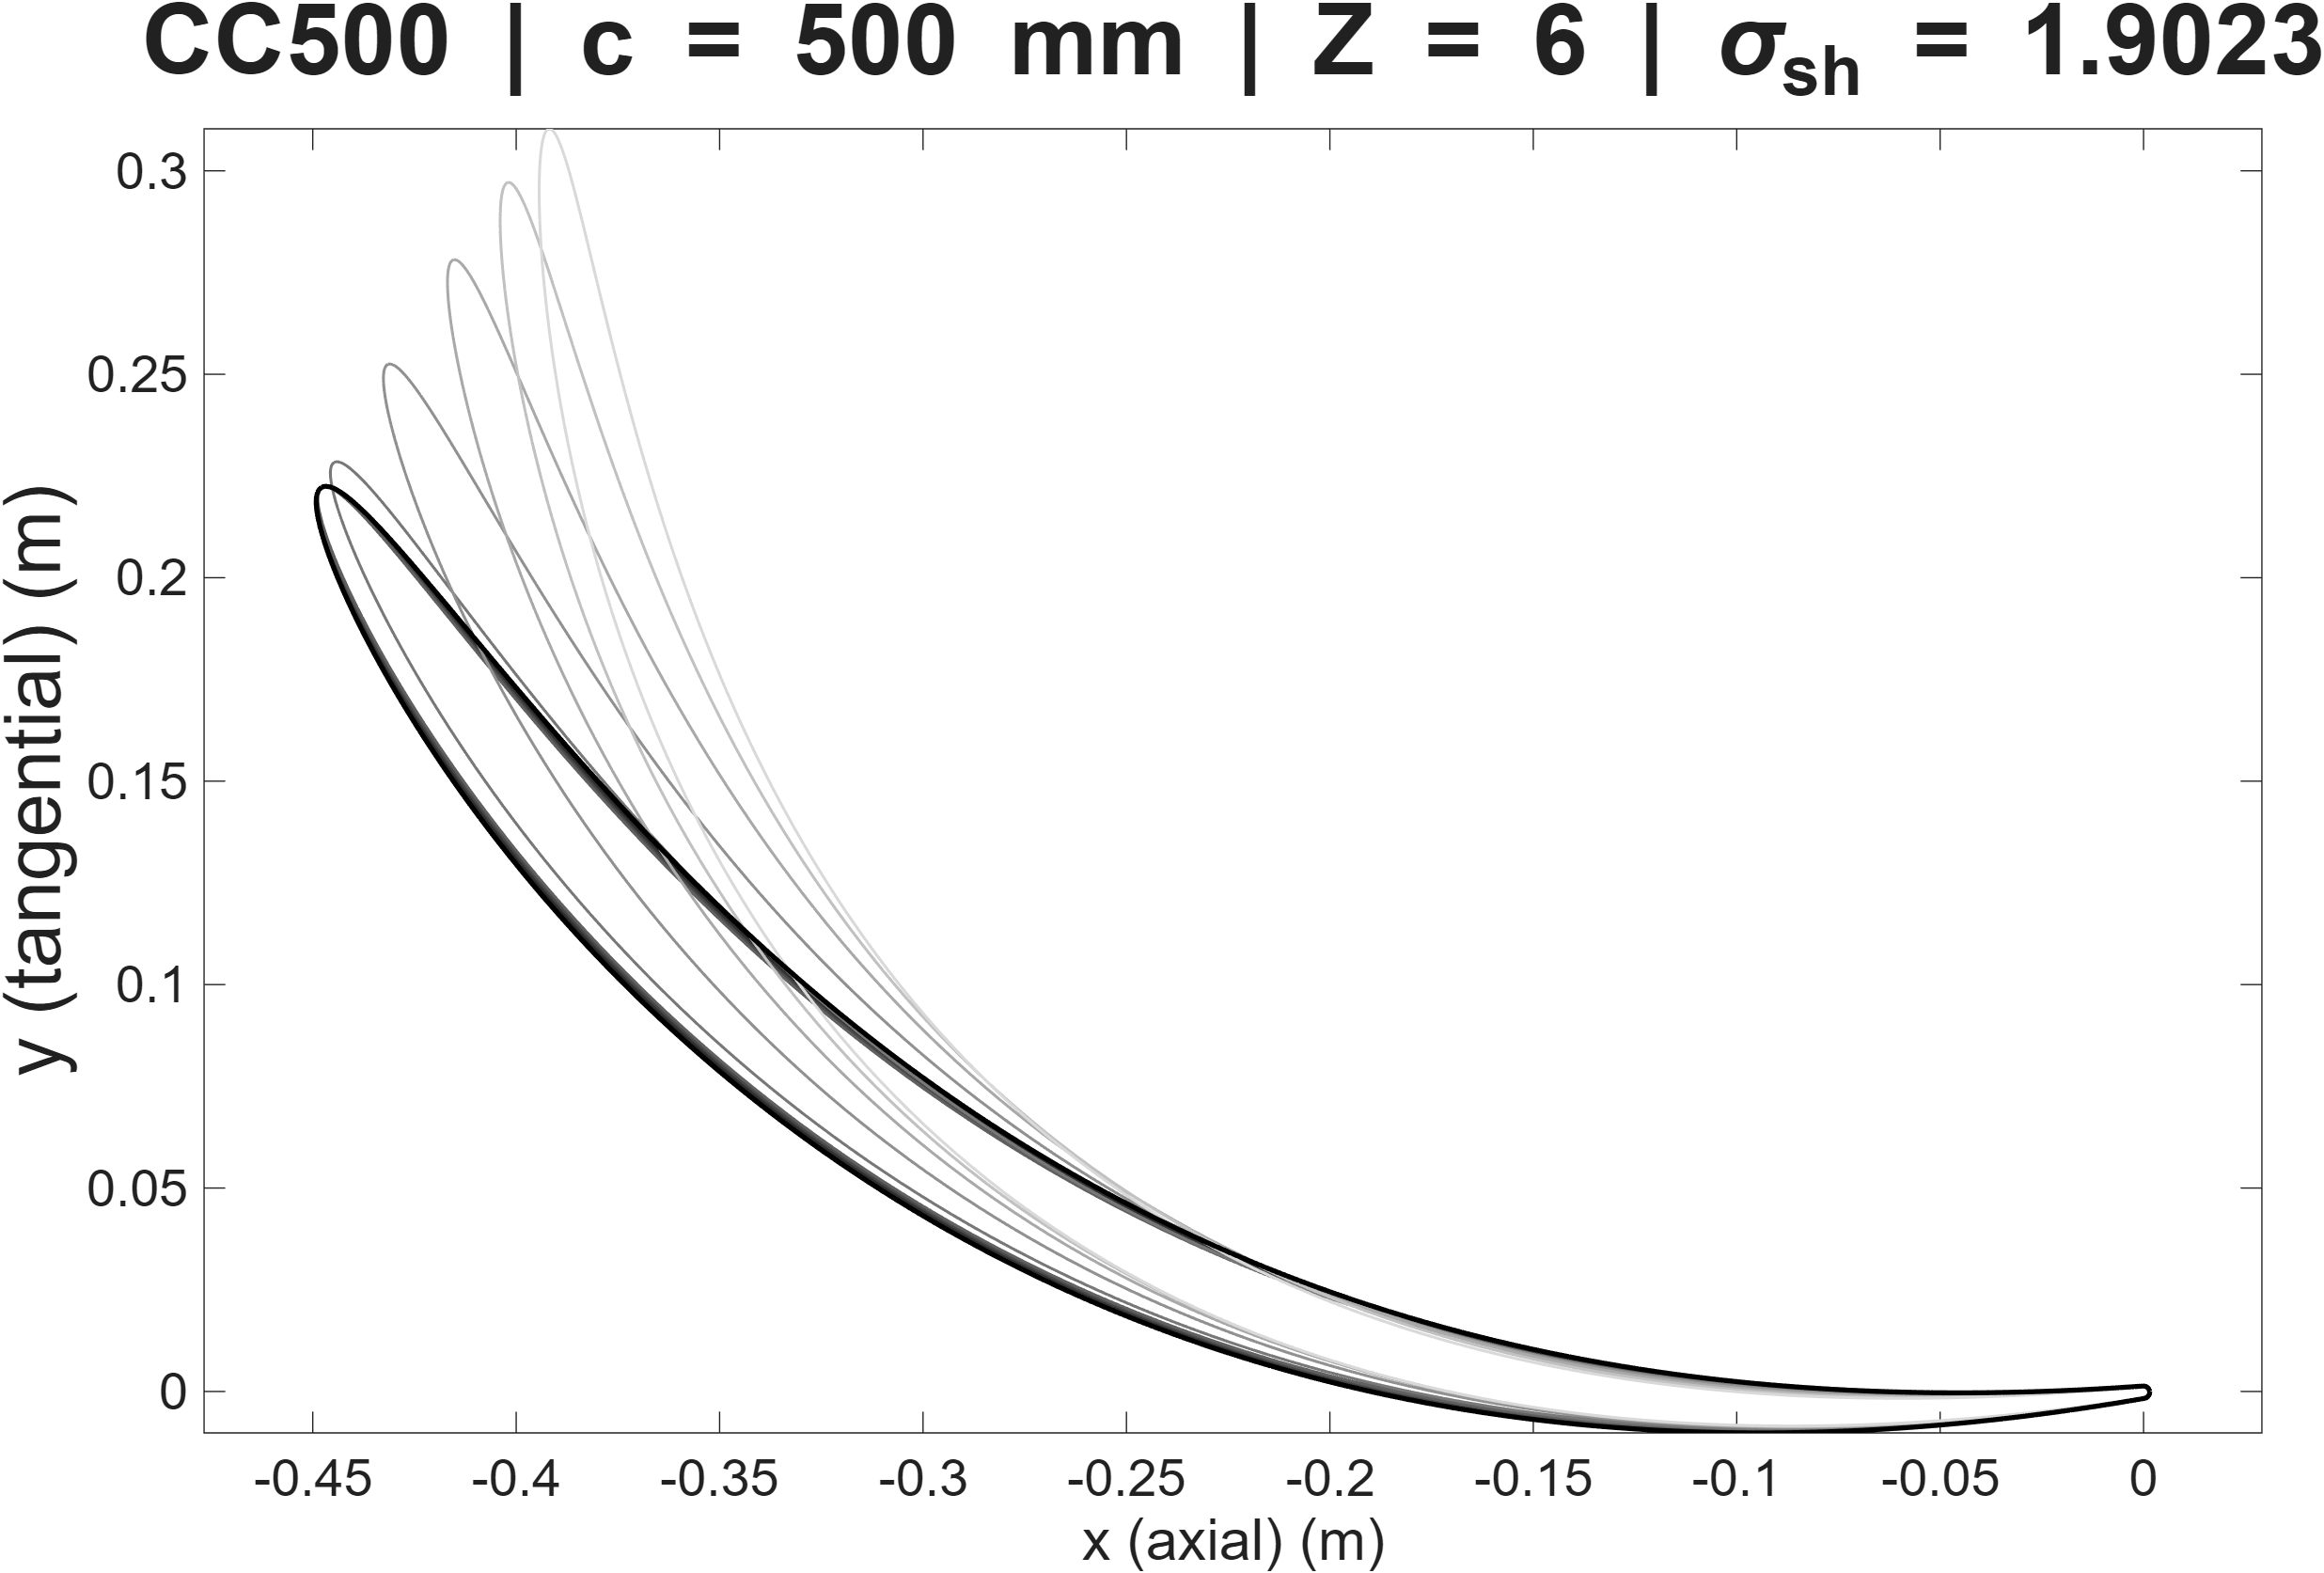
\includegraphics[width=\textwidth]{Figures/Foil2d/GV_Designs_2D/CC_500_6_2D.png}
    \caption{\texttt{CC\_500\_6}: $c = 500$~mm, $Z_s = 6$, $\sigma_{\mathrm{shroud}} = 1.90$.}
  \end{subfigure}

  \vspace{0.6em}

  \begin{subfigure}[b]{0.48\textwidth}
    \centering
    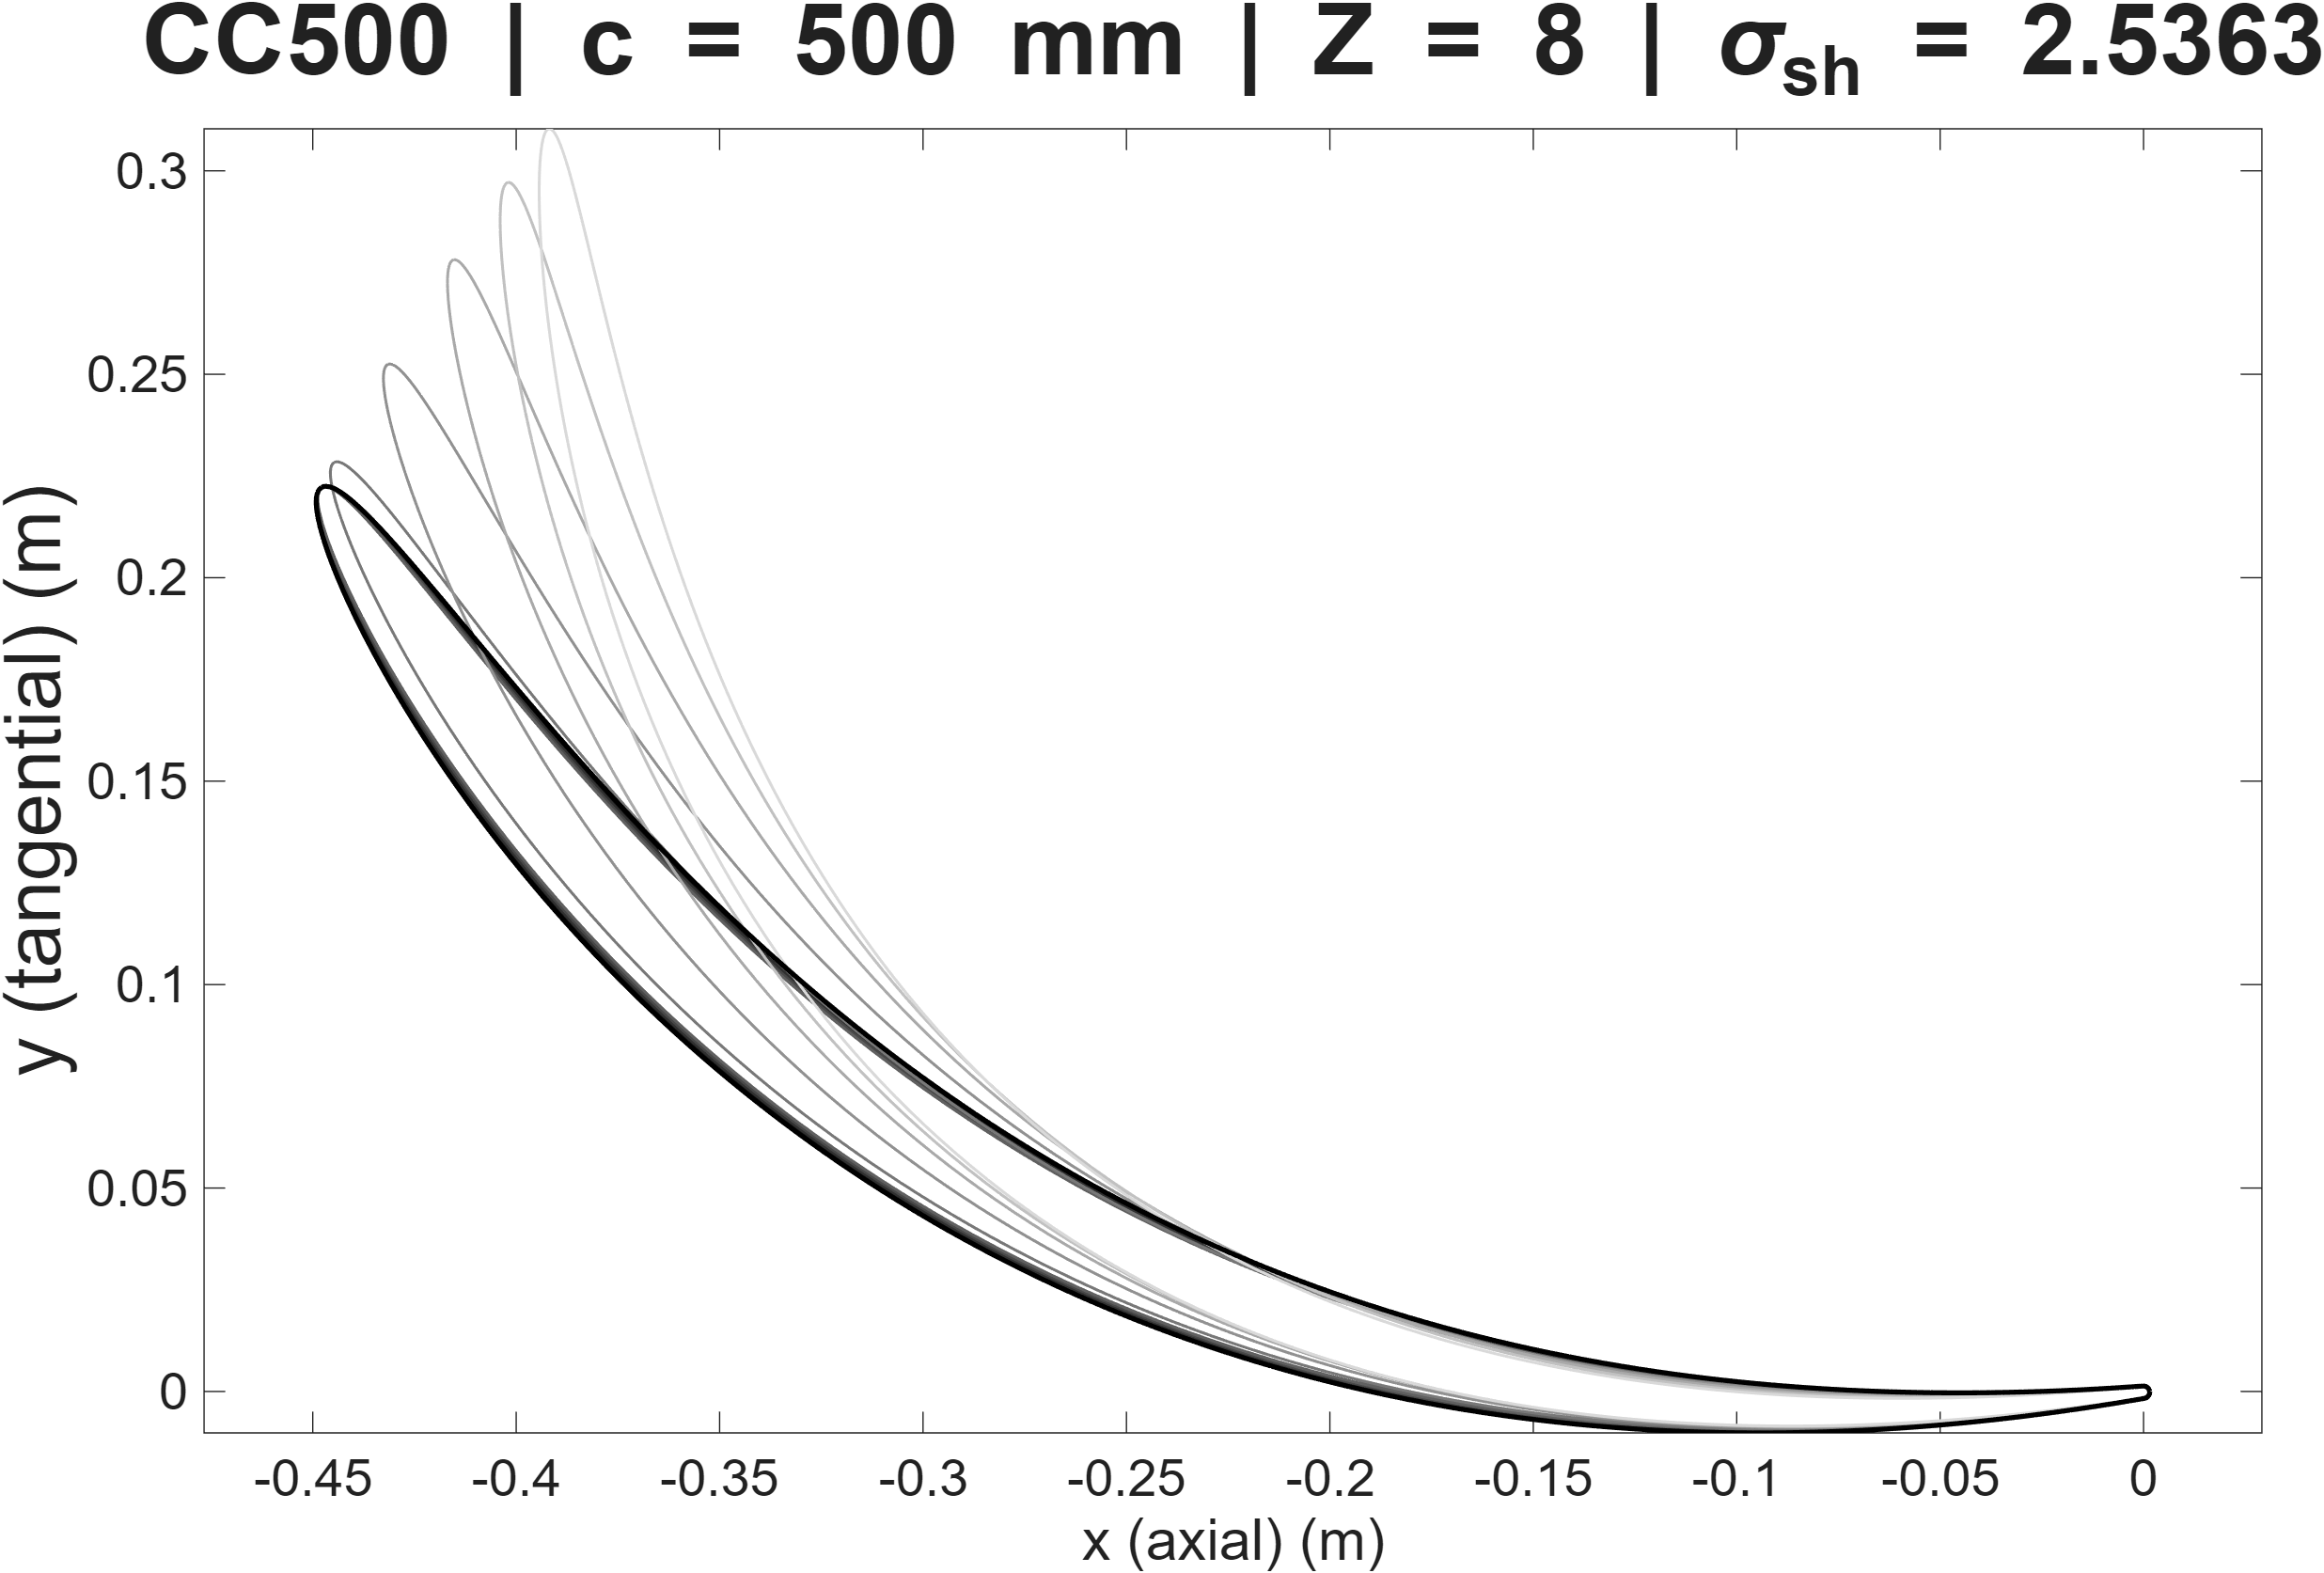
\includegraphics[width=\textwidth]{Figures/Foil2d/GV_Designs_2D/CC_500_8_2D.png}
    \caption{\texttt{CC\_500\_8}: $c = 500$~mm, $Z_s = 8$, $\sigma_{\mathrm{shroud}} = 2.54$.}
  \end{subfigure}

  \caption[CC family 2D sections, part 2 of 2]{Two-dimensional section stacks of the constant-chord (CC) family, configurations \texttt{CC\_450\_8} through \texttt{CC\_500\_8}. \texttt{CC\_500\_8} is the most heavily loaded configuration in the screening matrix.}
  \label{fig:cc_2d_2}
\end{figure}

\section*{Constant-solidity (CS) family}

\begin{figure}[H]
  \centering
  \begin{subfigure}[b]{0.48\textwidth}
    \centering
    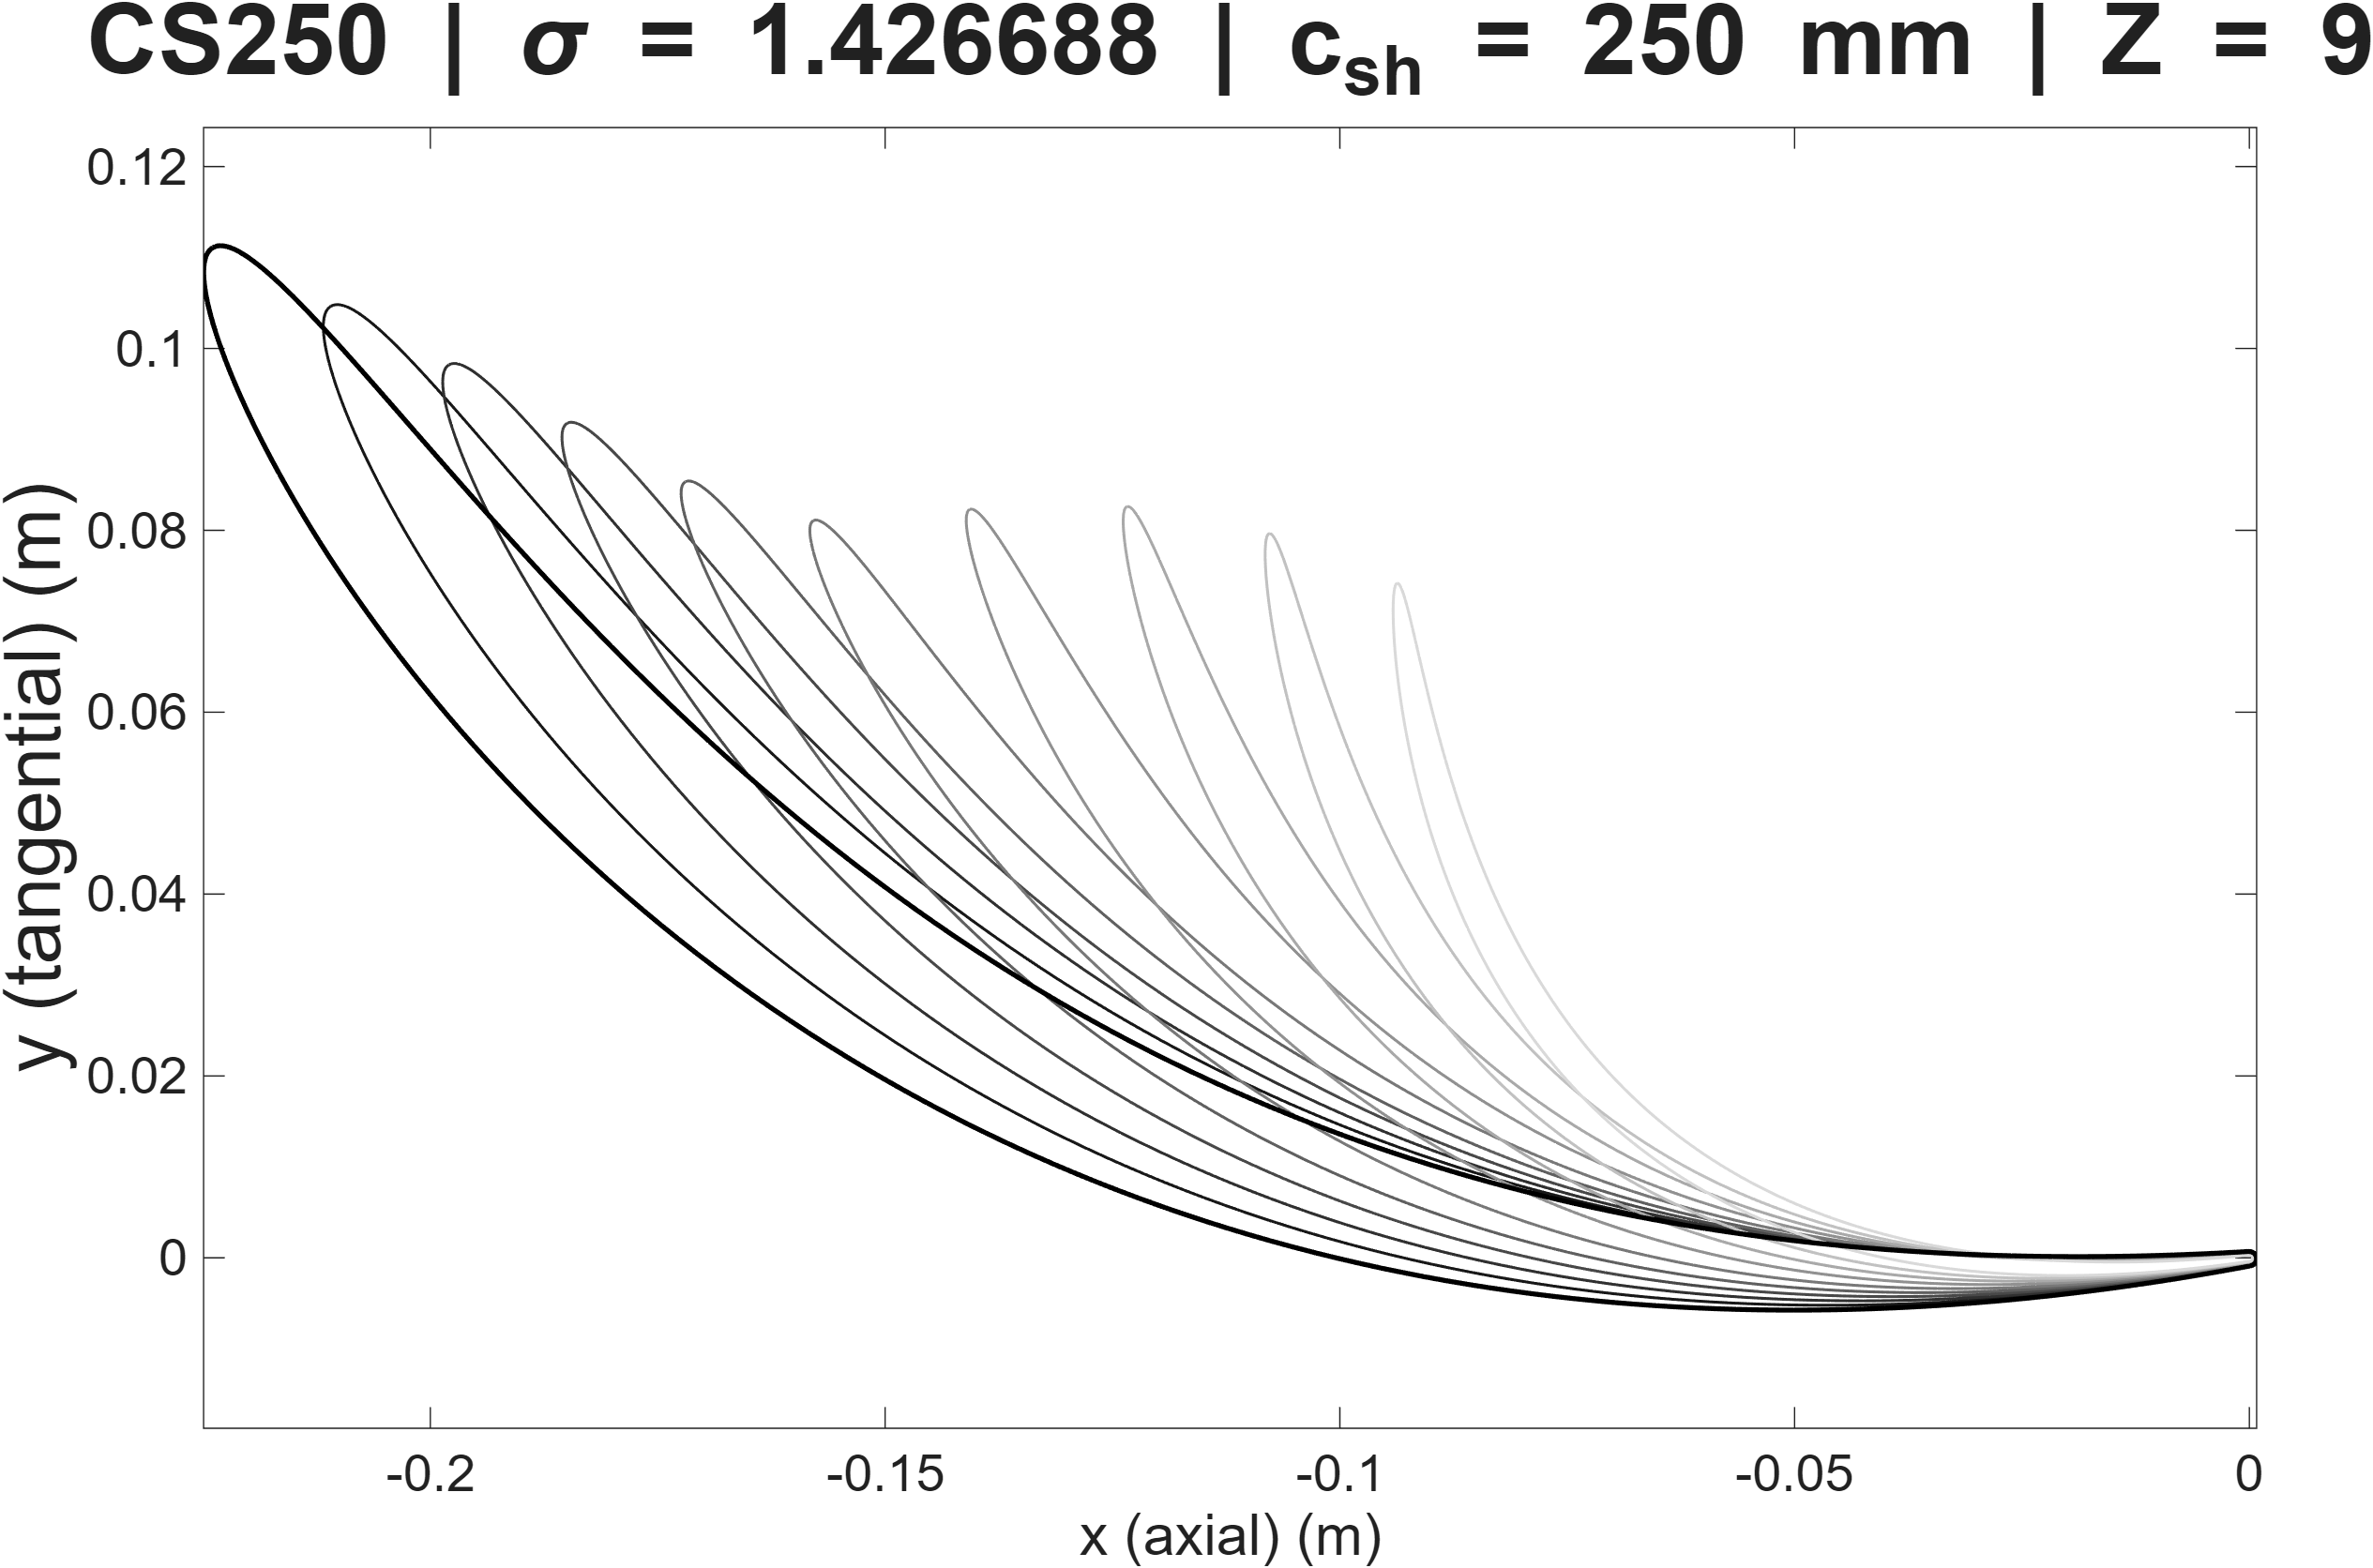
\includegraphics[width=\textwidth]{Figures/Foil2d/GV_Designs_2D/CS_250_9_2D.png}
    \caption{\texttt{CS\_250\_9}: $c_{\mathrm{shroud}} = 250$~mm, $Z_s = 9$, $\sigma = 1.43$ uniform.}
  \end{subfigure}
  \hfill
  \begin{subfigure}[b]{0.48\textwidth}
    \centering
    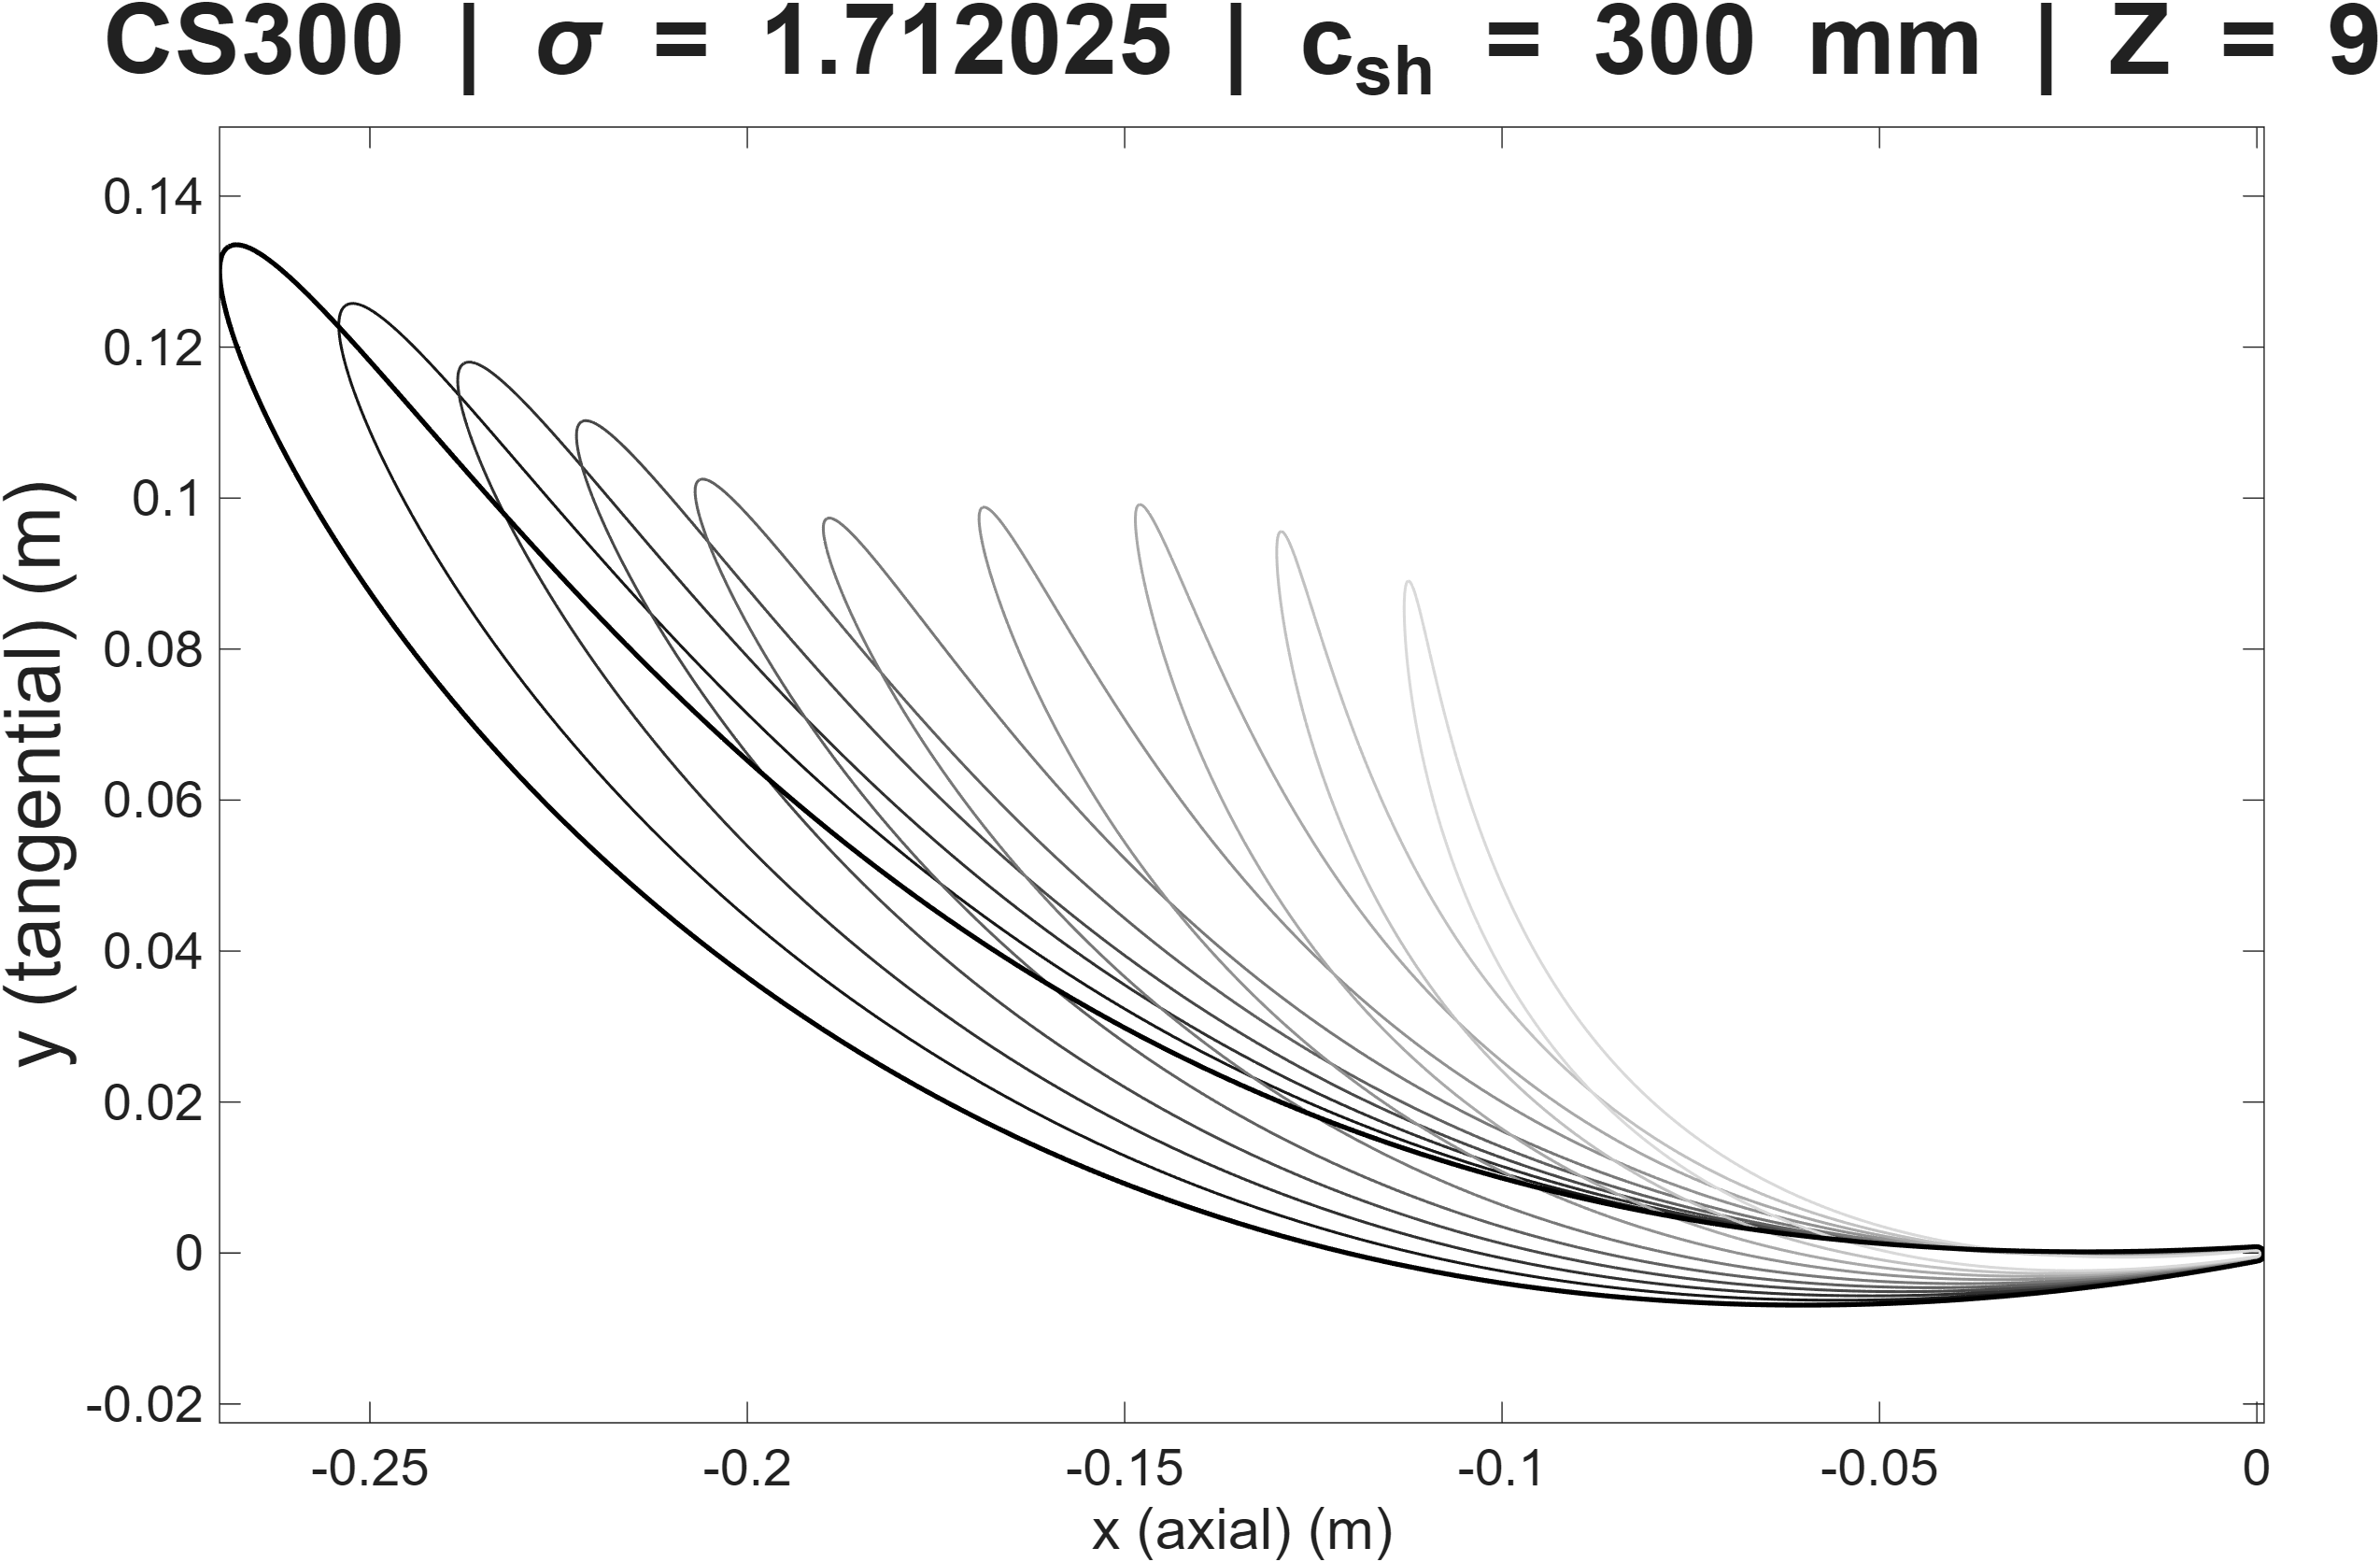
\includegraphics[width=\textwidth]{Figures/Foil2d/GV_Designs_2D/CS_300_9_2D.png}
    \caption{\texttt{CS\_300\_9}: $c_{\mathrm{shroud}} = 300$~mm, $Z_s = 9$, $\sigma = 1.71$ uniform.}
  \end{subfigure}

  \vspace{0.6em}

  \begin{subfigure}[b]{0.48\textwidth}
    \centering
    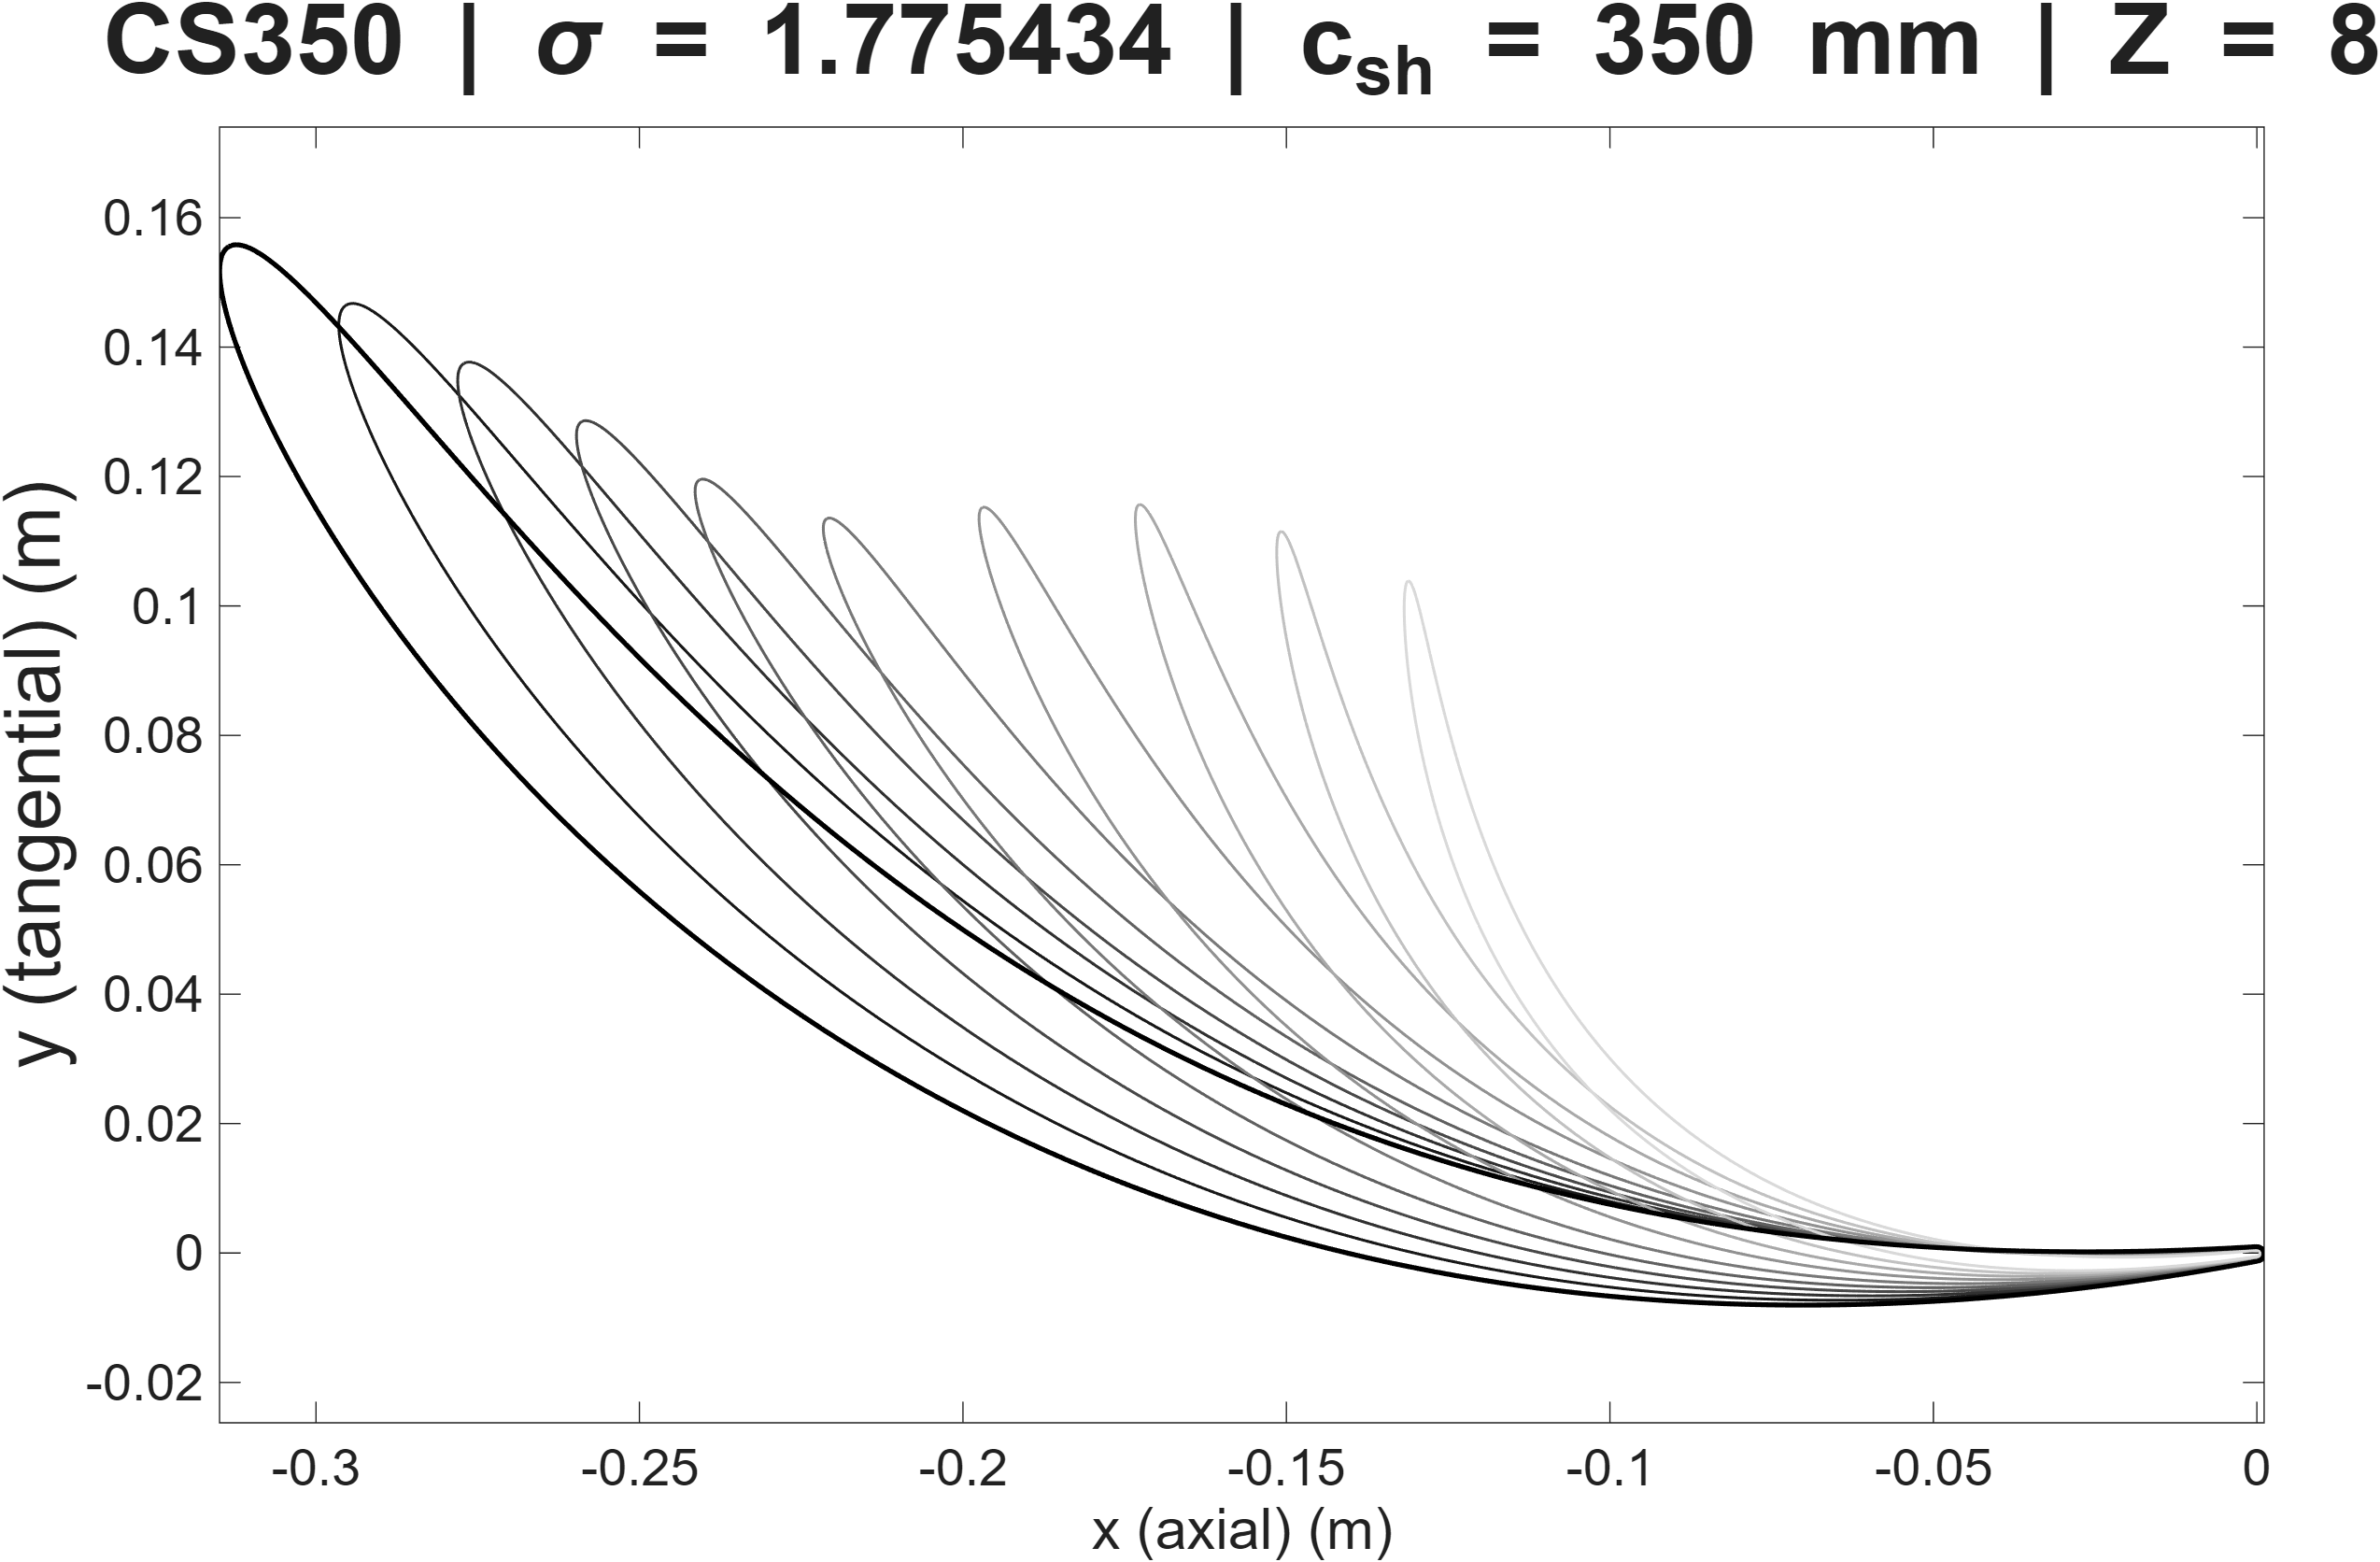
\includegraphics[width=\textwidth]{Figures/Foil2d/GV_Designs_2D/CS_350_8_2D.png}
    \caption{\texttt{CS\_350\_8}: $c_{\mathrm{shroud}} = 350$~mm, $Z_s = 8$, $\sigma = 1.78$ uniform.}
  \end{subfigure}
  \hfill
  \begin{subfigure}[b]{0.48\textwidth}
    \centering
    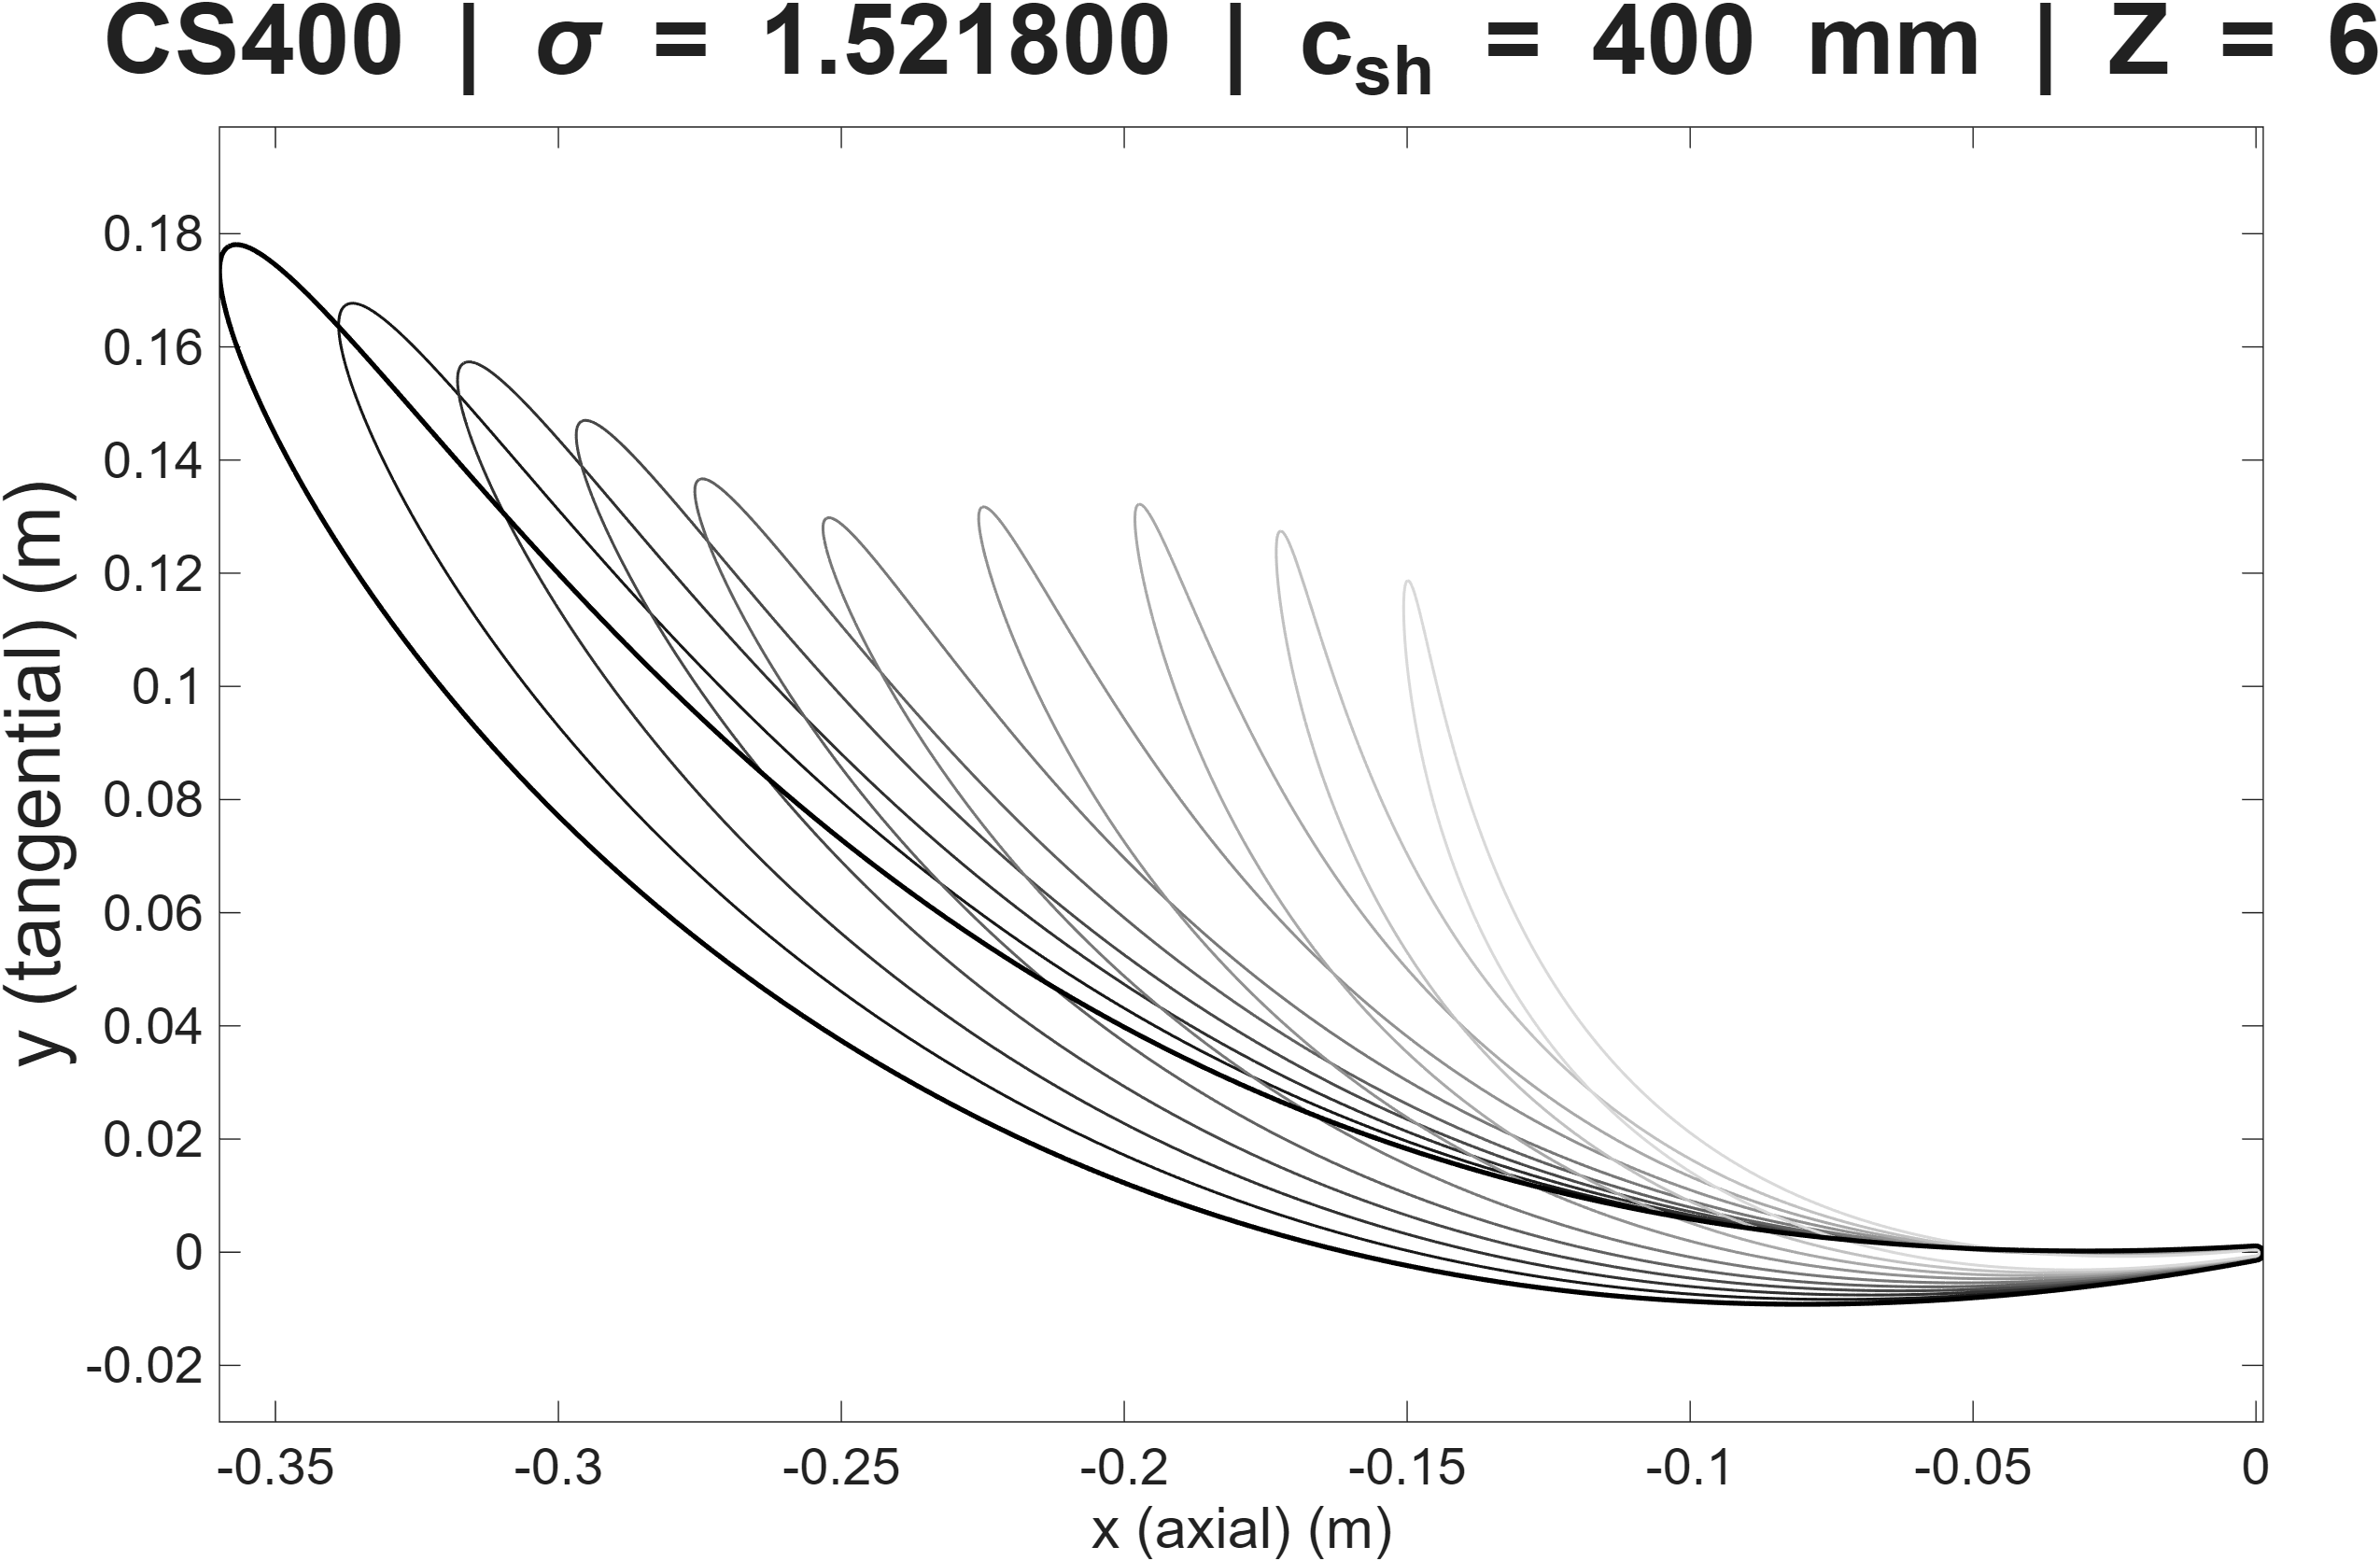
\includegraphics[width=\textwidth]{Figures/Foil2d/GV_Designs_2D/CS_400_6_2D.png}
    \caption{\texttt{CS\_400\_6}: $c_{\mathrm{shroud}} = 400$~mm, $Z_s = 6$, $\sigma = 1.52$ uniform.}
  \end{subfigure}

  \vspace{0.6em}

  \begin{subfigure}[b]{0.48\textwidth}
    \centering
    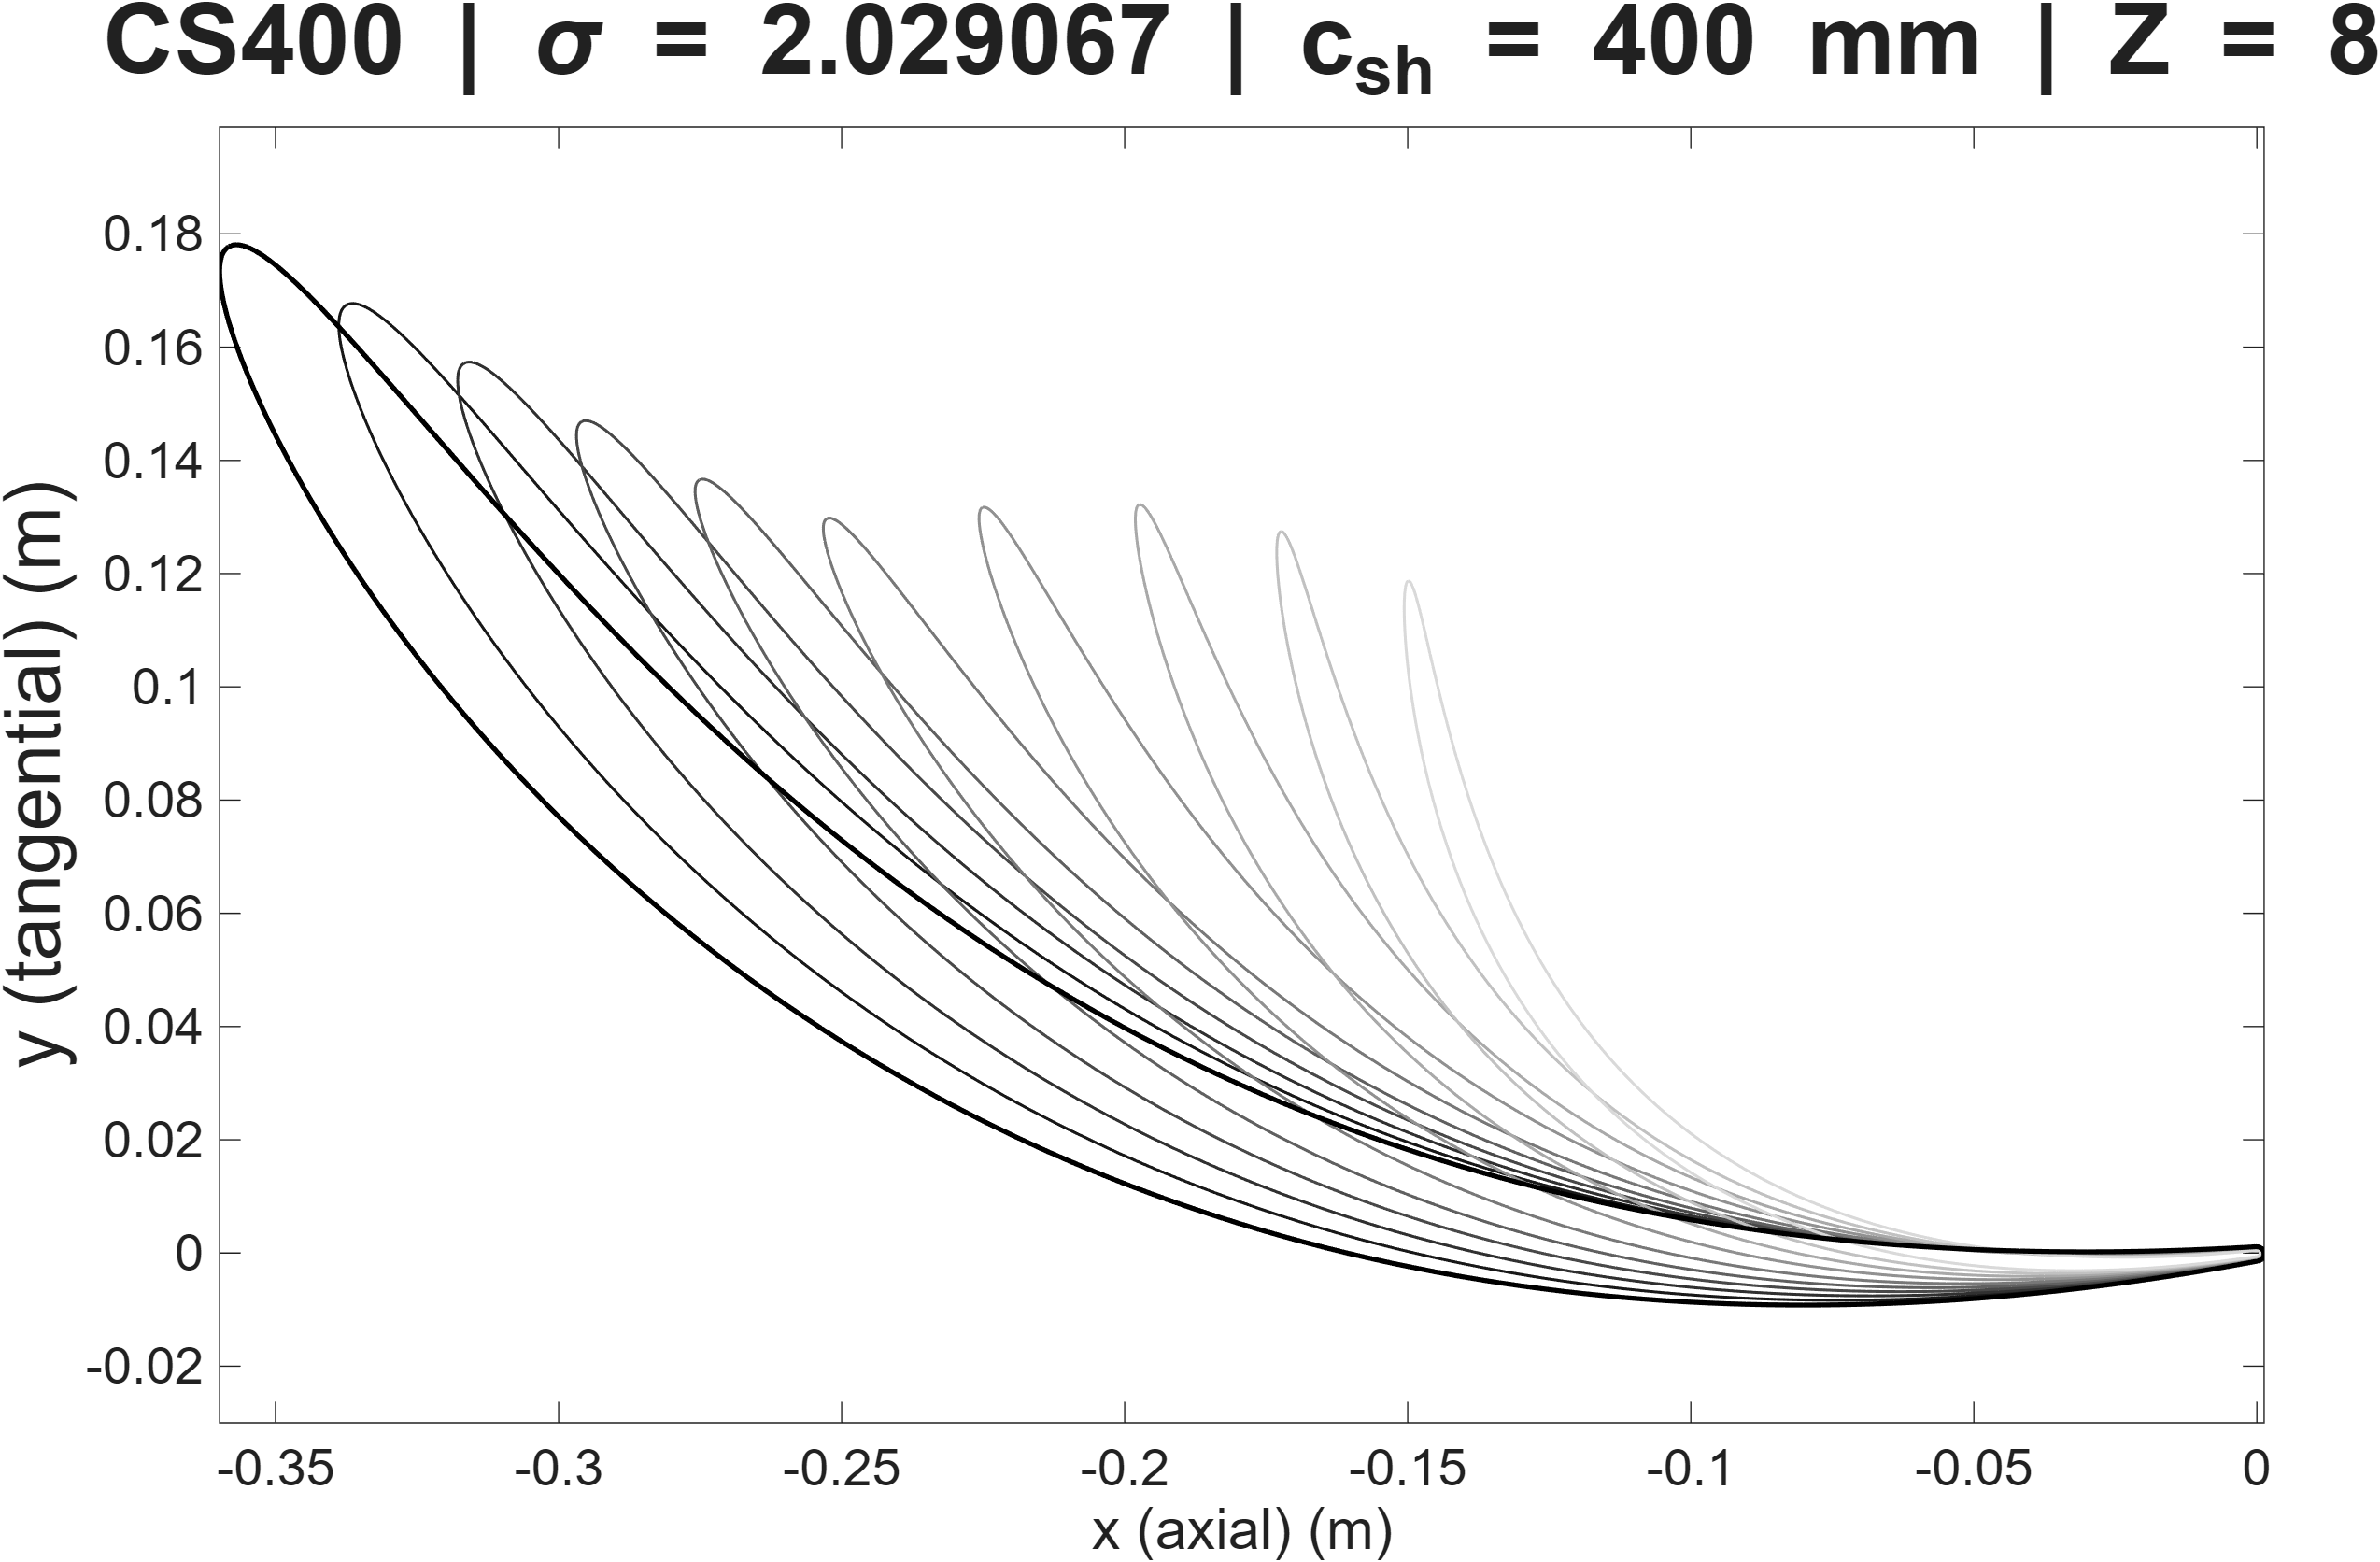
\includegraphics[width=\textwidth]{Figures/Foil2d/GV_Designs_2D/CS_400_8_2D.png}
    \caption{\texttt{CS\_400\_8}: $c_{\mathrm{shroud}} = 400$~mm, $Z_s = 8$, $\sigma = 2.03$ uniform.}
  \end{subfigure}
  \hfill
  \begin{subfigure}[b]{0.48\textwidth}
    \centering
    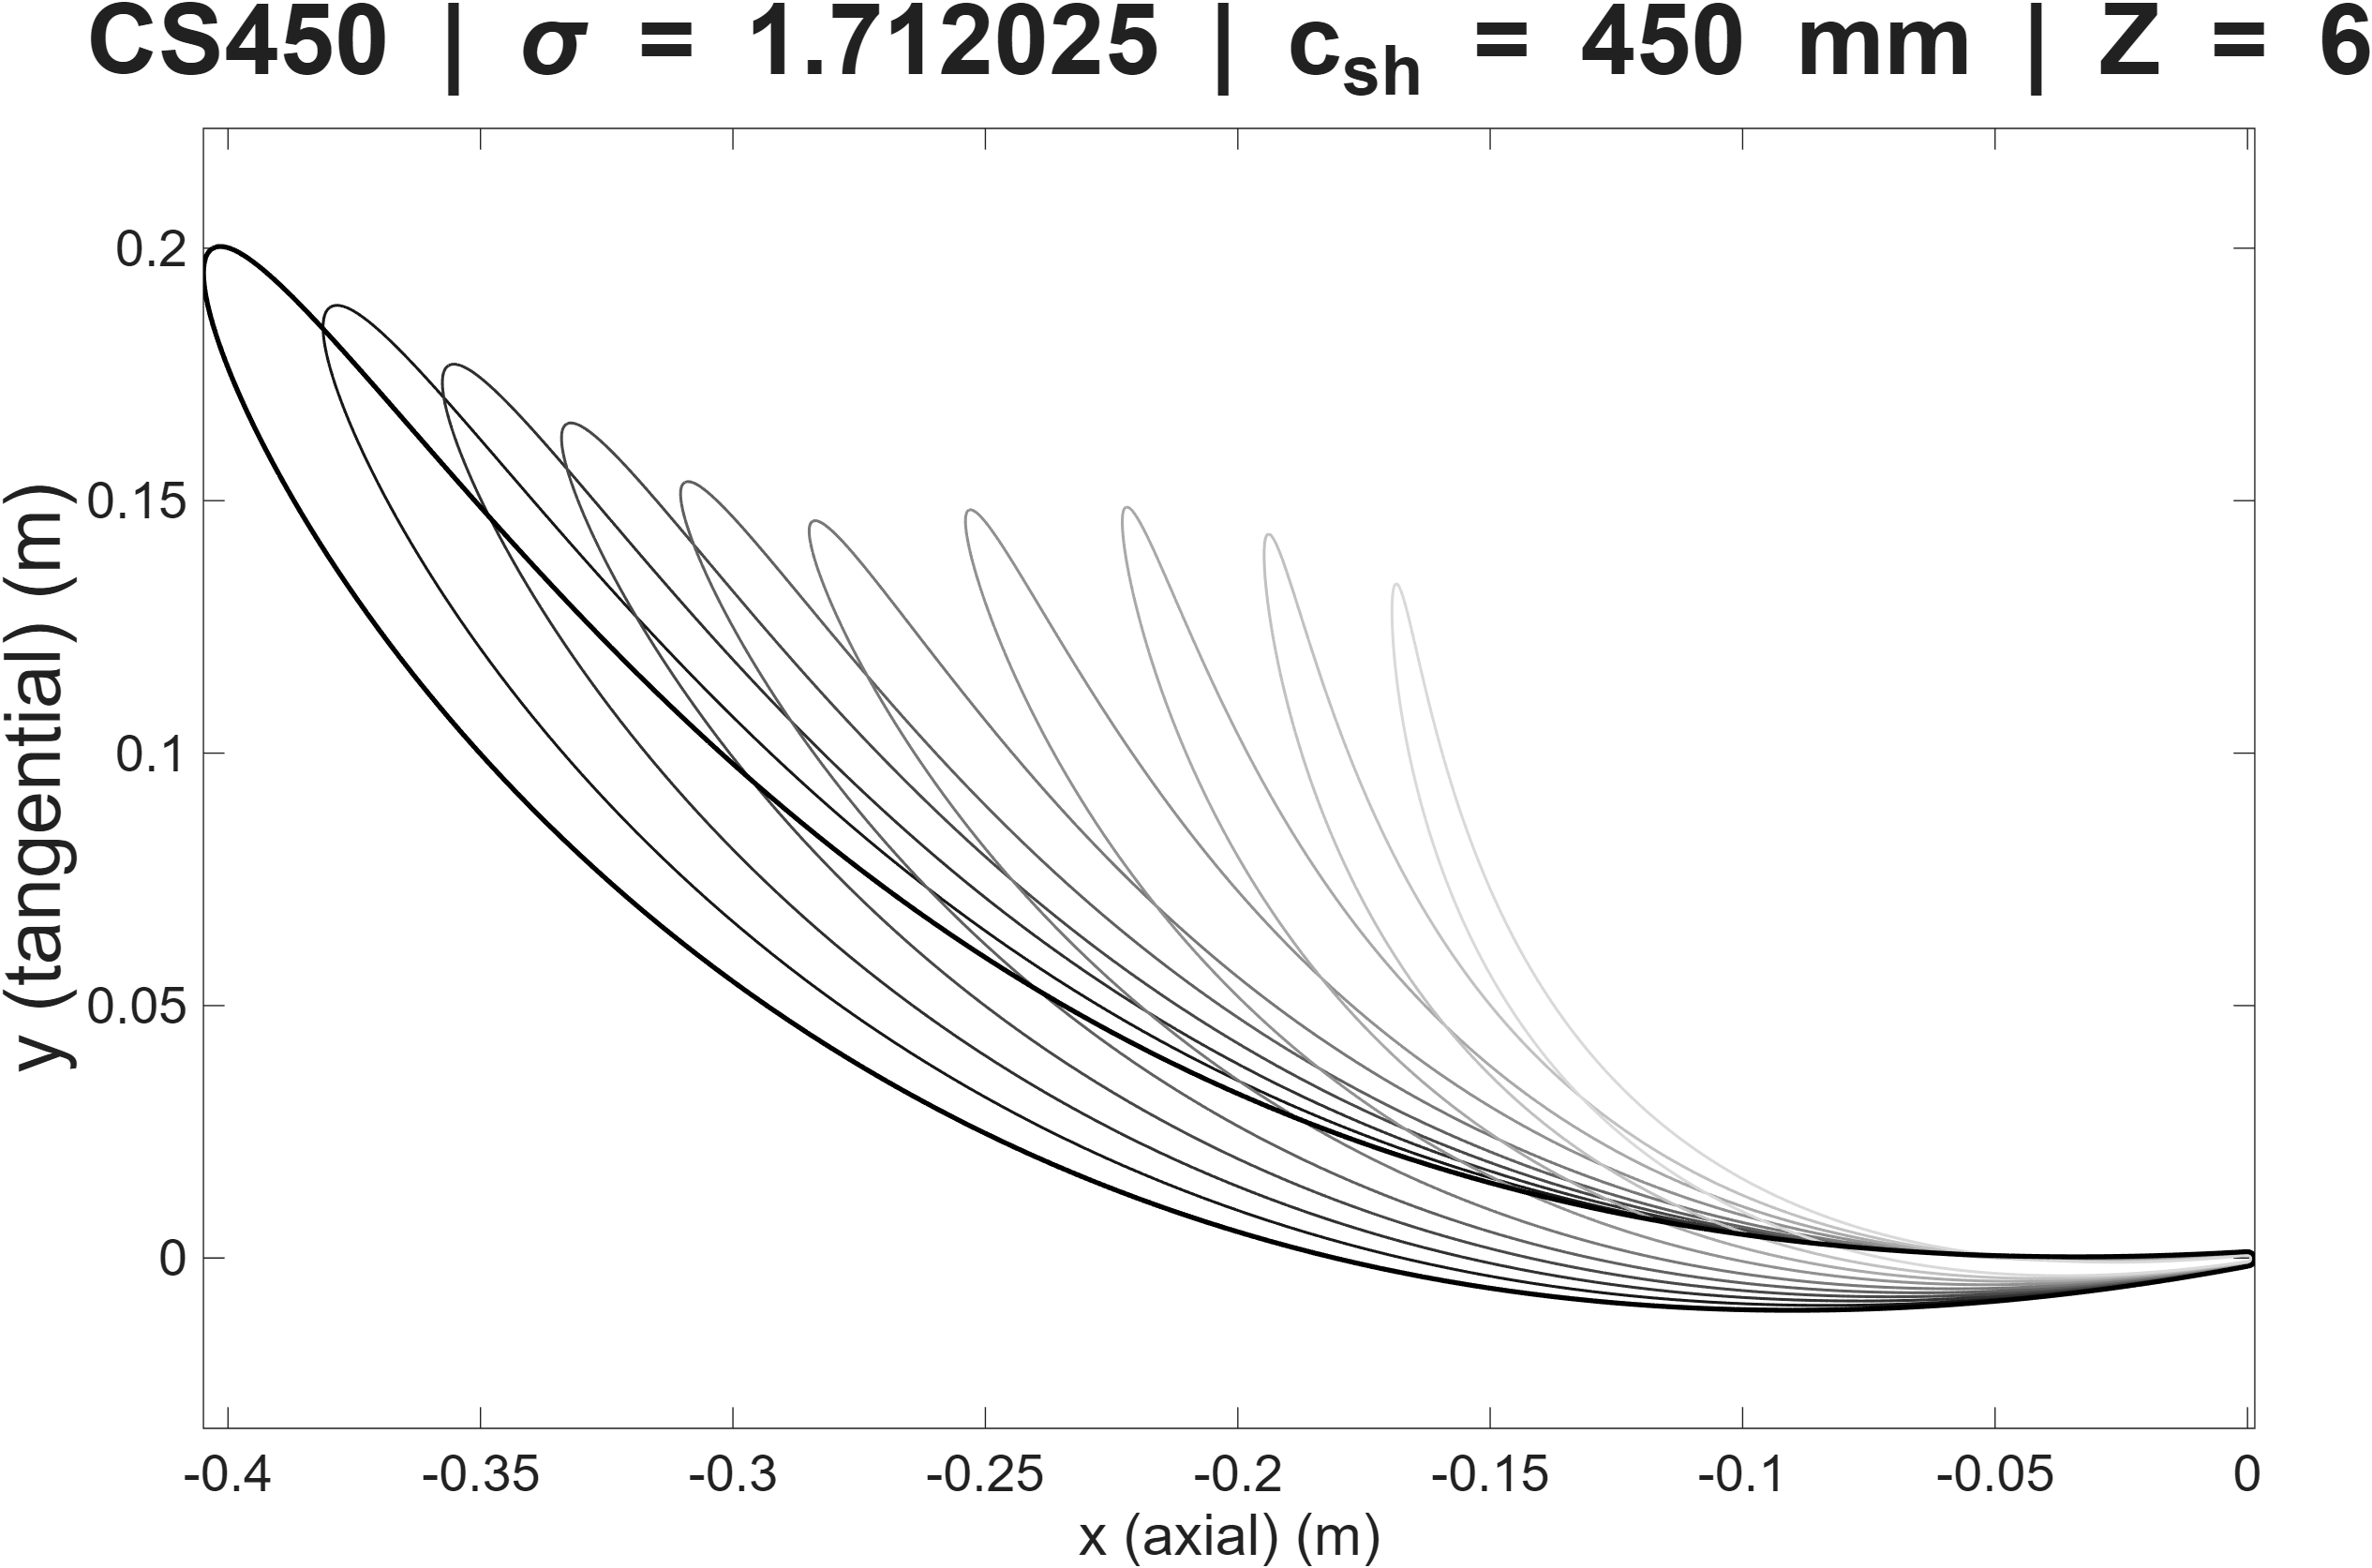
\includegraphics[width=\textwidth]{Figures/Foil2d/GV_Designs_2D/CS_450_6_2D.png}
    \caption{\texttt{CS\_450\_6}: $c_{\mathrm{shroud}} = 450$~mm, $Z_s = 6$, $\sigma = 1.71$ uniform.}
  \end{subfigure}

  \caption[CS family 2D sections, part 1 of 2]{Two-dimensional section stacks of the constant-solidity (CS) family, configurations \texttt{CS\_250\_9} through \texttt{CS\_450\_6}. The chord scales linearly with $r$, so the sections taper inwards and the inner outlines are shorter than the shroud section.}
  \label{fig:cs_2d_1}
\end{figure}

\begin{figure}[H]
  \centering
  \begin{subfigure}[b]{0.48\textwidth}
    \centering
    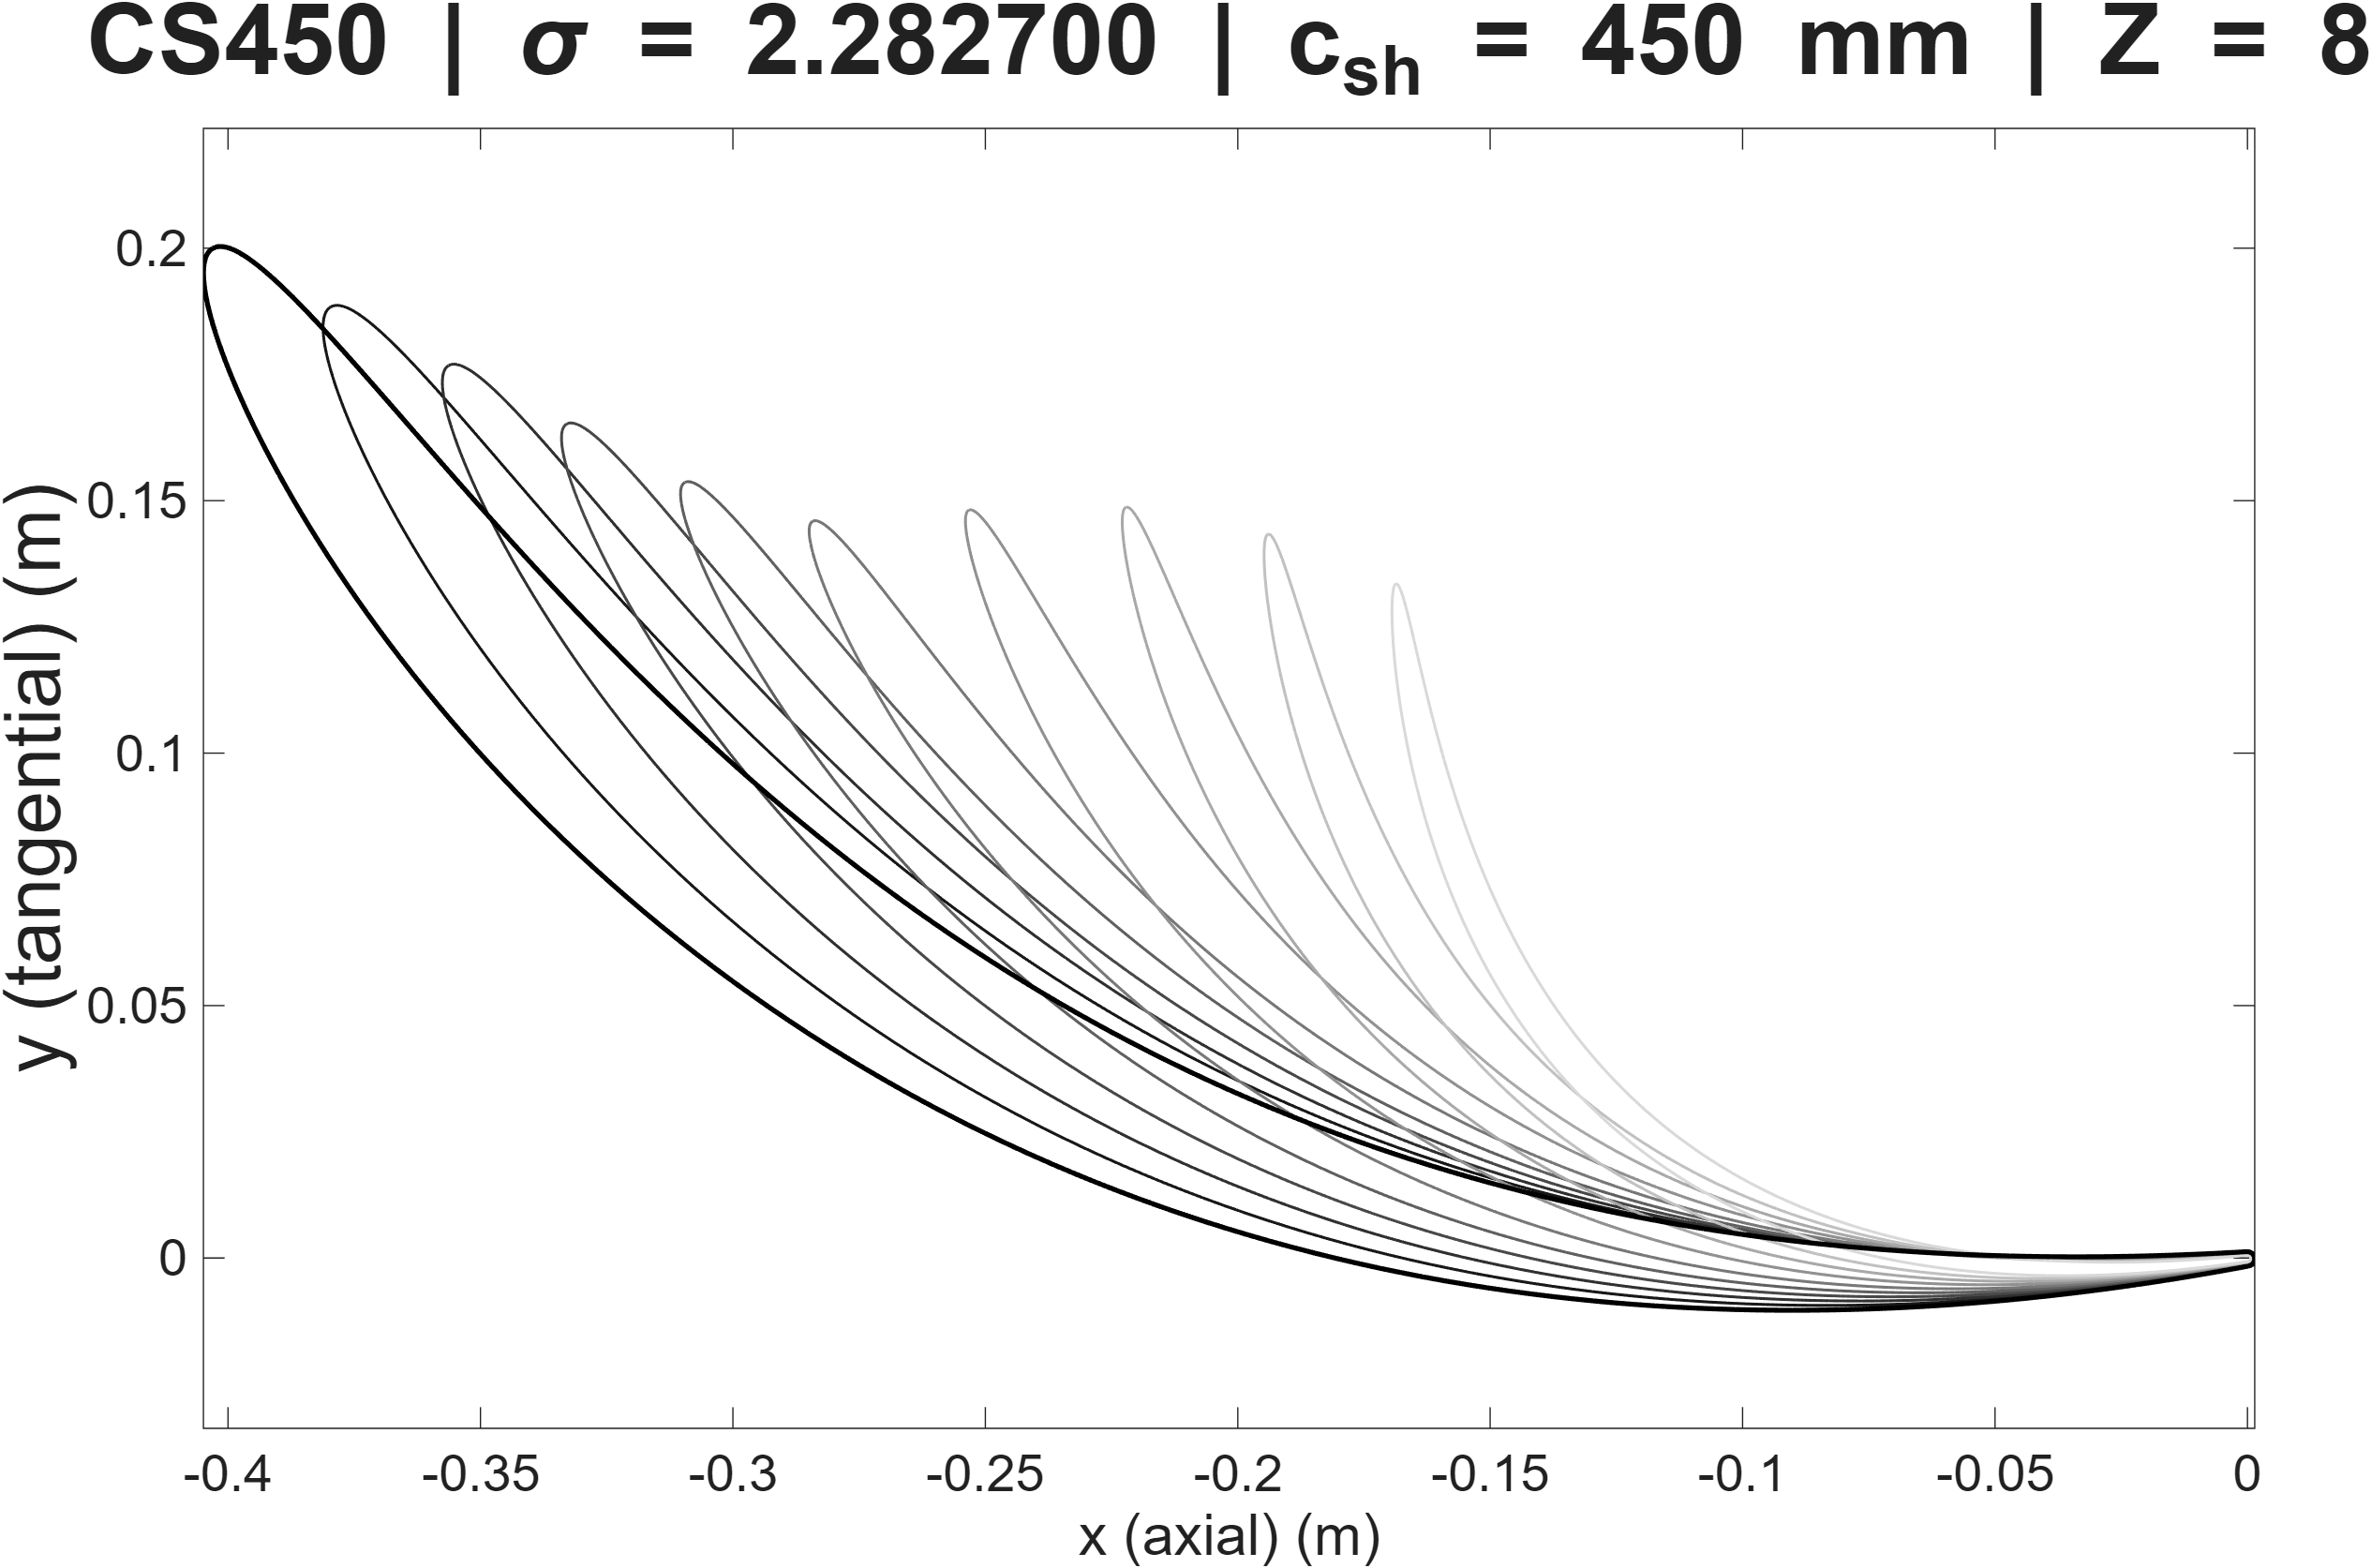
\includegraphics[width=\textwidth]{Figures/Foil2d/GV_Designs_2D/CS_450_8_2D.png}
    \caption{\texttt{CS\_450\_8}: $c_{\mathrm{shroud}} = 450$~mm, $Z_s = 8$, $\sigma = 2.28$ uniform.}
  \end{subfigure}
  \hfill
  \begin{subfigure}[b]{0.48\textwidth}
    \centering
    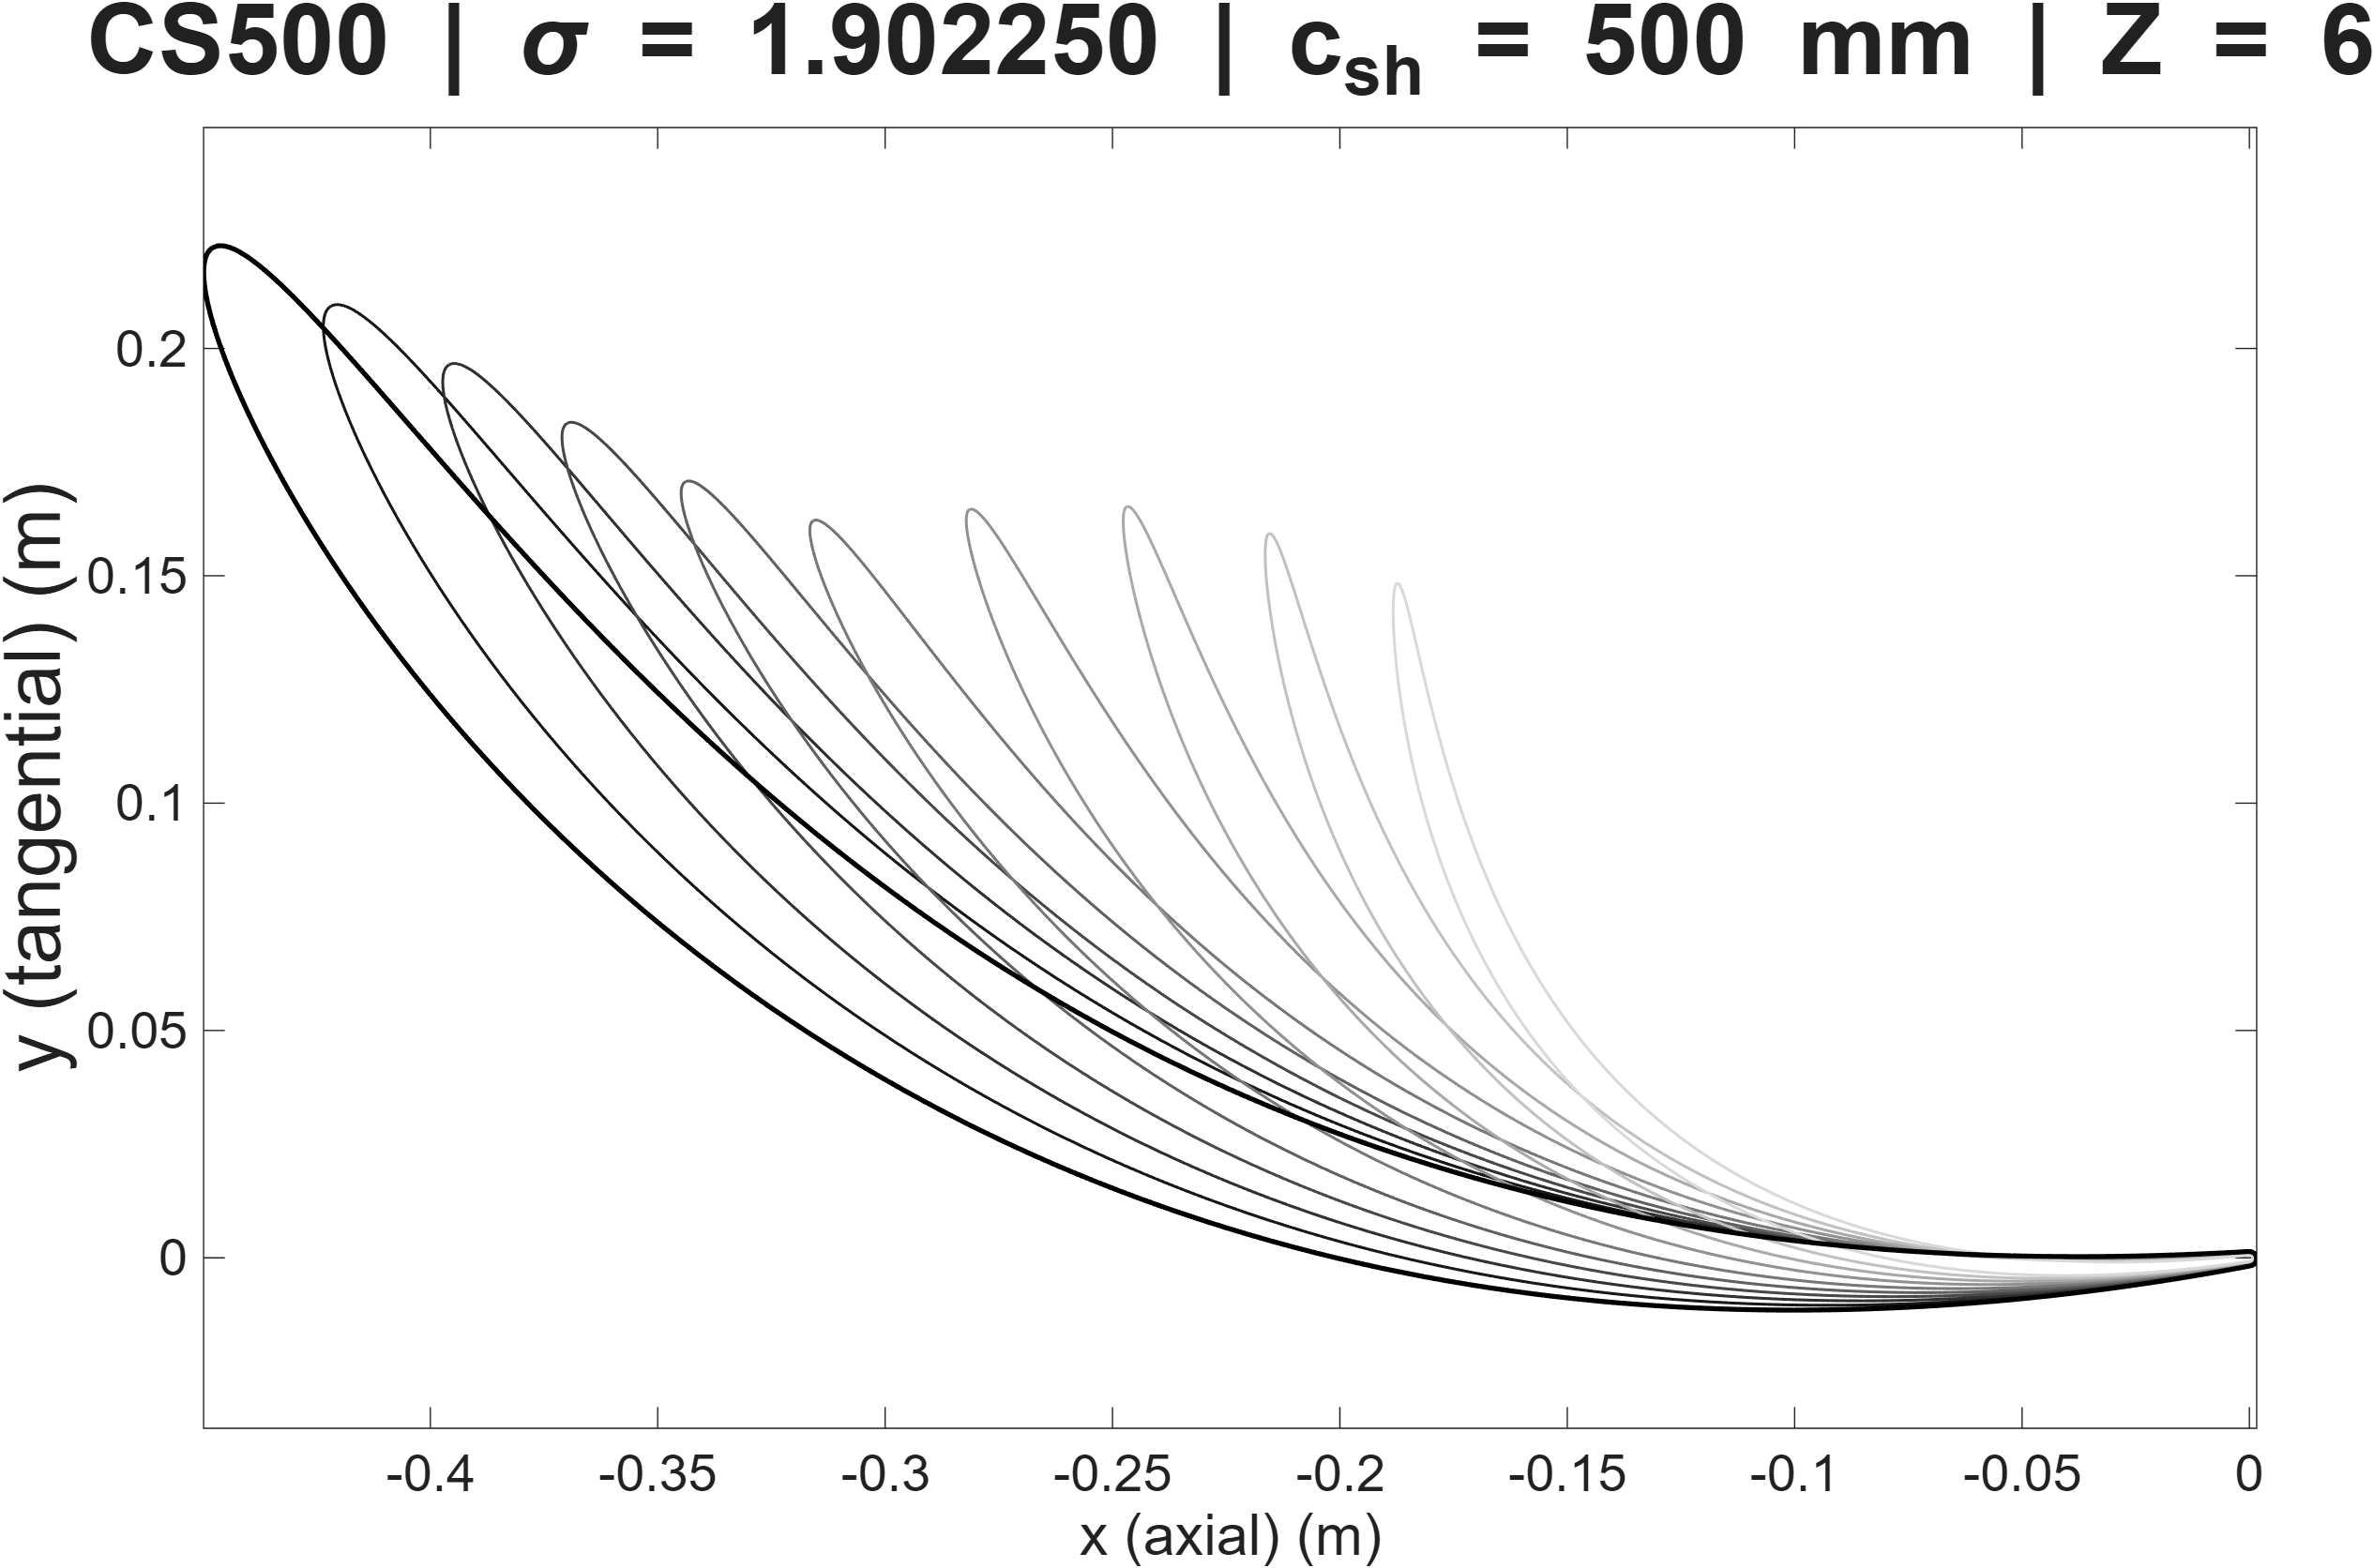
\includegraphics[width=\textwidth]{Figures/Foil2d/GV_Designs_2D/CS_500_6_2D.png}
    \caption{\texttt{CS\_500\_6}: $c_{\mathrm{shroud}} = 500$~mm, $Z_s = 6$, $\sigma = 1.90$ uniform.}
  \end{subfigure}

  \vspace{0.6em}

  \begin{subfigure}[b]{0.48\textwidth}
    \centering
    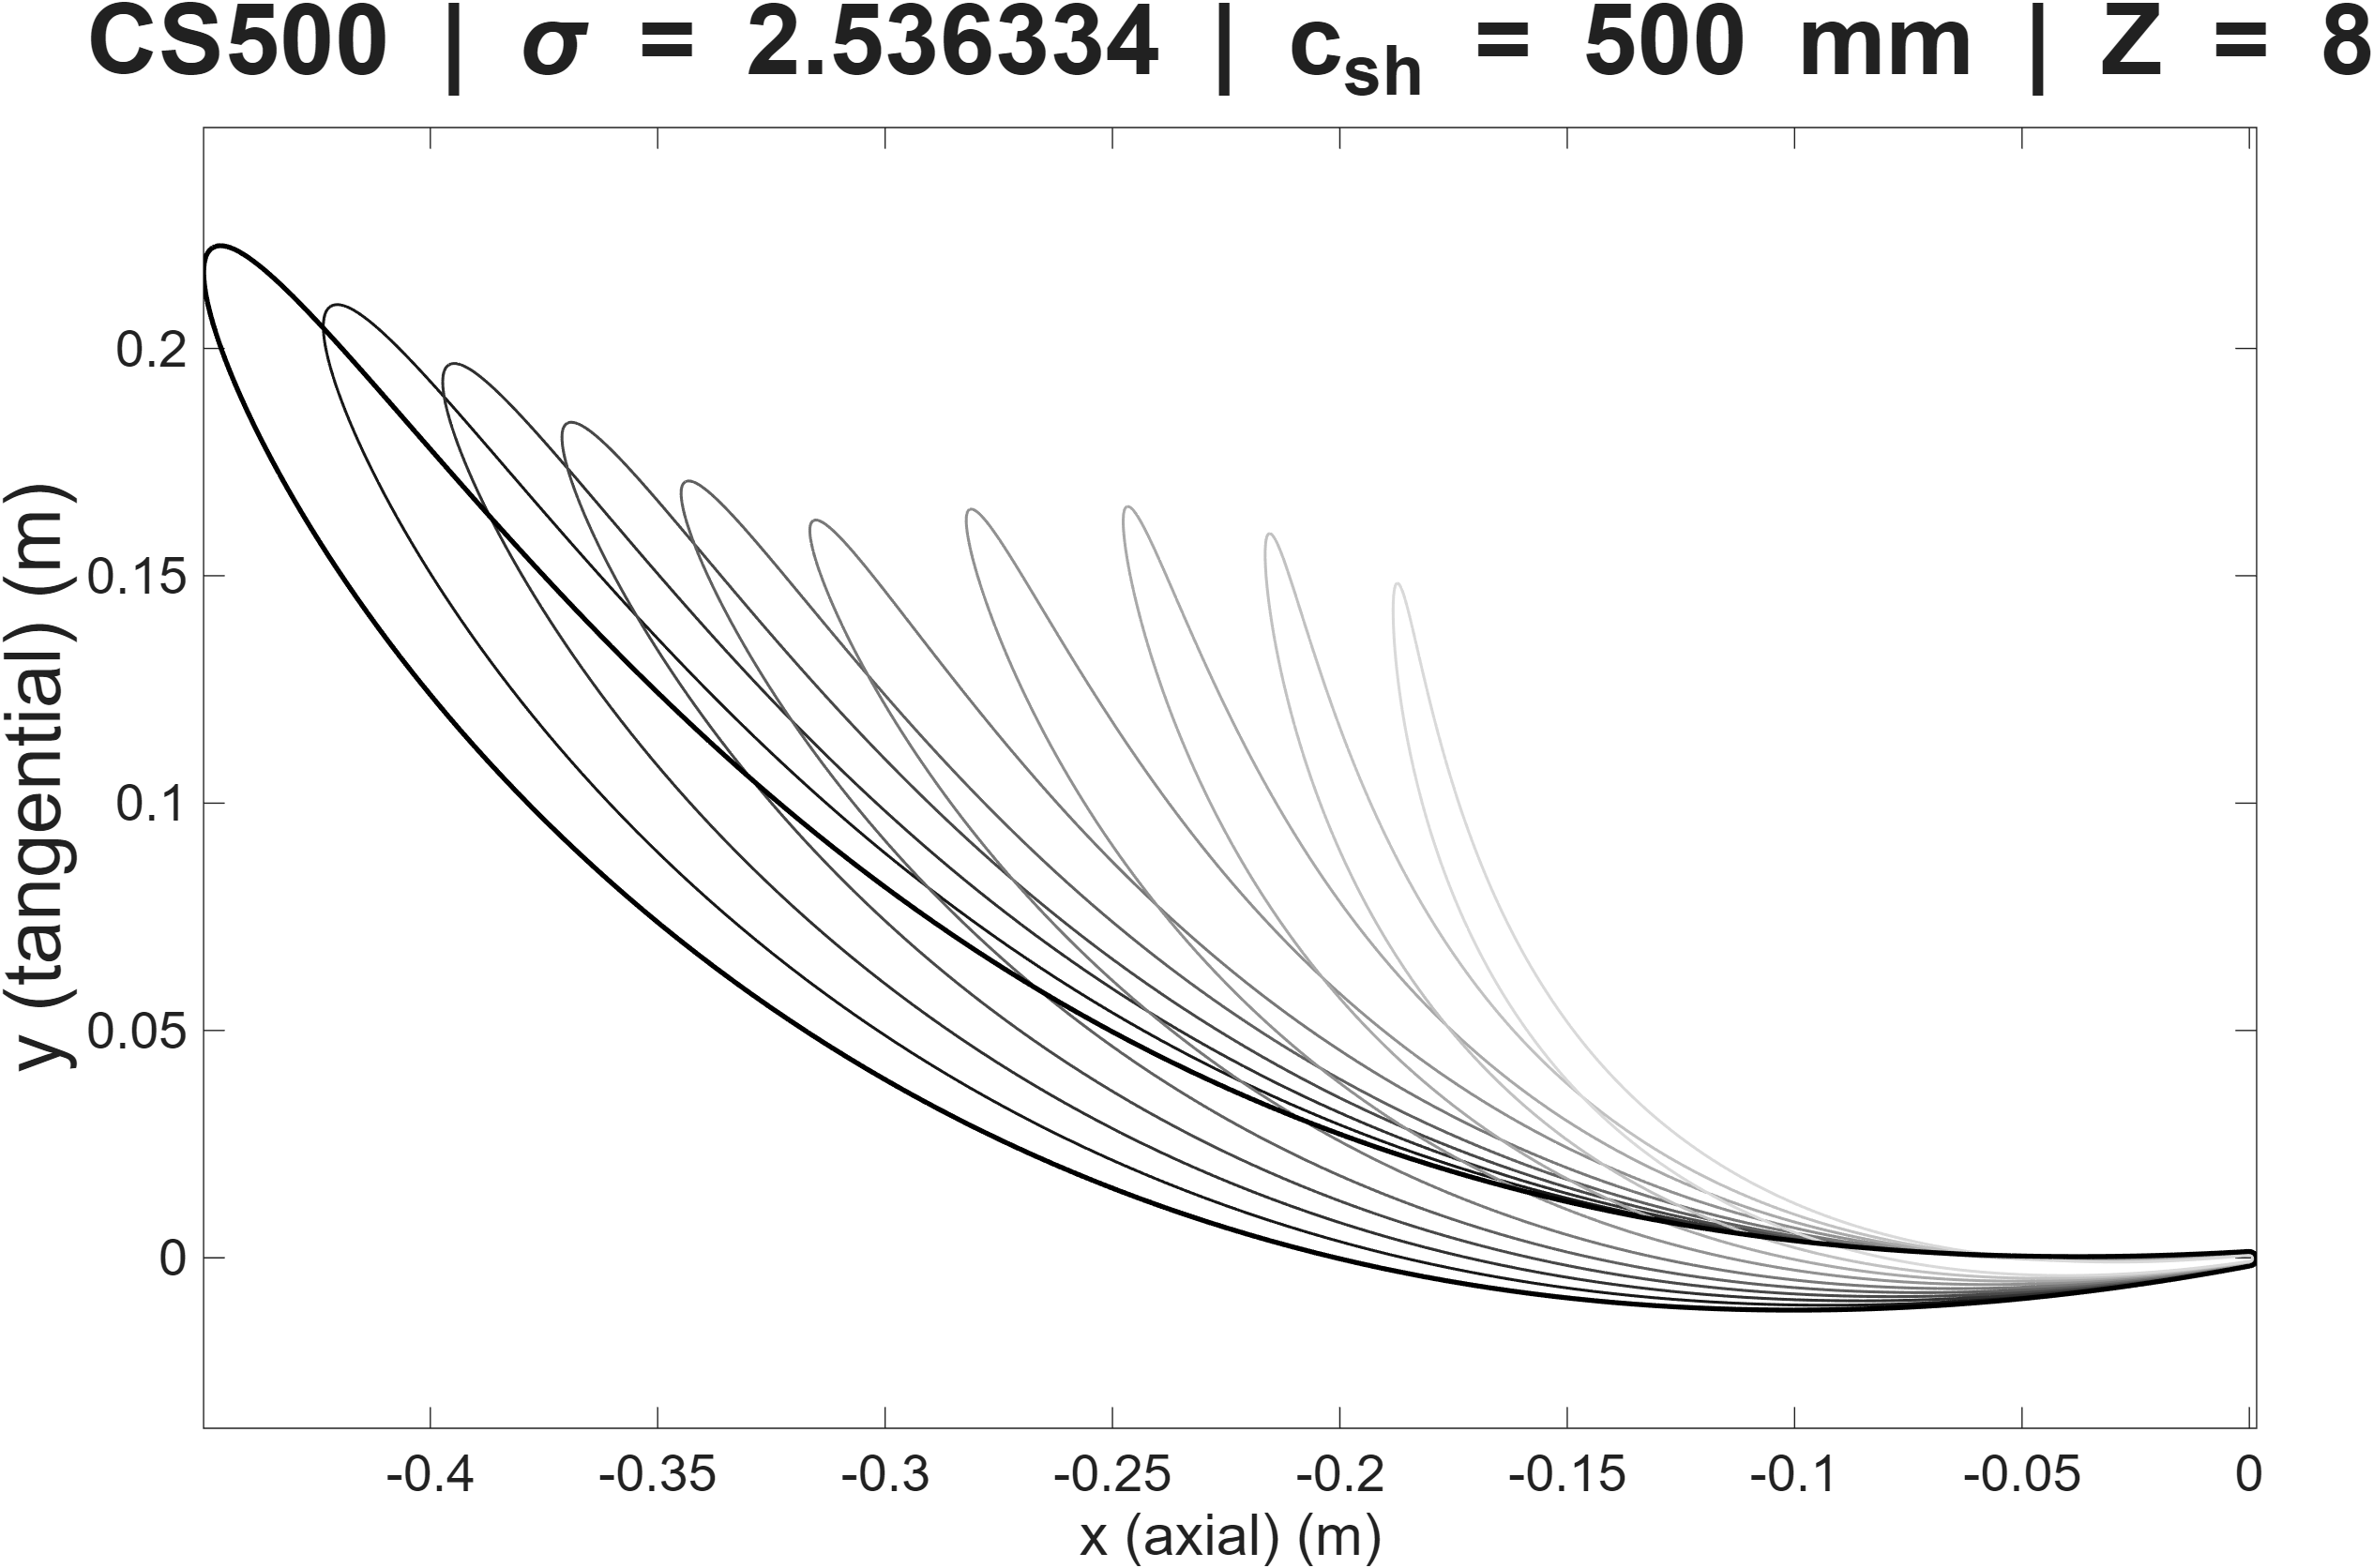
\includegraphics[width=\textwidth]{Figures/Foil2d/GV_Designs_2D/CS_500_8_2D.png}
    \caption{\texttt{CS\_500\_8}: $c_{\mathrm{shroud}} = 500$~mm, $Z_s = 8$, $\sigma = 2.54$ uniform.}
  \end{subfigure}

  \caption[CS family 2D sections, part 2 of 2]{Two-dimensional section stacks of the constant-solidity (CS) family, configurations \texttt{CS\_450\_8} through \texttt{CS\_500\_8}.}
  \label{fig:cs_2d_2}
\end{figure}

%DEAR HÅVARD 10.06: (new content) Nytt Appendix E med de 18 2D-seksjonene fra Figures/Foil2d/GV_Designs_2D/ (var ubrukt). Strukturert som Appendix B (CC foer CS, sortert paa korde og skovltall). Siden denne fila (Appendix-E.tex) naa har \chapter igjen, rykker Q-criterion (Appendix-F.tex) tilbake til bokstav F, saa filnavn = bokstav stemmer for A-F. G/H/I er fortsatt tomme. La ogsaa inn EN kryssreferanse i Ch3 (sec:theory_const_chord_const_sol) til dette appendikset. sigma_shroud-verdiene i bildetekstene er hentet fra Appendix B for konsistens; plottittelen i hver figur oppgir c, Z og sigma uansett.
\clearpage % Keep this at the end of the chapter
